\documentclass{article}
\usepackage[utf8]{inputenc}
\usepackage[margin=2cm]{geometry}
\usepackage{amsmath, amssymb}
\usepackage{bm}
\usepackage{lineno}
\renewcommand\linenumberfont{\normalfont\bfseries\small\color{darkgrey}}
\usepackage{booktabs}
\usepackage[round]{natbib}
\bibliographystyle{plainnat}
\usepackage{authblk}
% Linux Libertine:
\usepackage{textcomp}
\usepackage[sb]{libertine}
\usepackage[varqu,varl]{inconsolata}% sans serif typewriter
\usepackage[libertine,bigdelims,vvarbb]{newtxmath} % bb from STIX
\usepackage[cal=boondoxo]{mathalfa} % mathcal
\useosf % osf for text, not math
\usepackage[supstfm=libertinesups,%
  supscaled=1.2,%
  raised=-.13em]{superiors}
\usepackage{setspace}
\usepackage{siunitx}
\usepackage[section]{placeins} % Keep floats (figs, tabs, eqns) in the right section
% I assume these all work together to make nice colour
\usepackage[dvipsnames]{xcolor}
\definecolor{niceblue}{HTML}{236899} % Depends \usepackage[dvipsnames]{xcolor}
\definecolor{darkgrey}{HTML}{A9A9A9} % Depends \usepackage[dvipsnames]{xcolor}
\usepackage{hyperref}
\hypersetup{
    colorlinks=true,
    linkcolor=black,
    filecolor=black,      
    urlcolor=niceblue,
    citecolor=niceblue,
    linkbordercolor = white
}
% End nice colour
\usepackage{pgfplotstable} % For tables
\pgfplotsset{compat=1.16} % For tables
\newcommand{\yearStart}{1979}
\newcommand{\yearEnd}{2017}
\newcommand{\nYears}{39}
\newcommand{\nRegionsThree}{3}
\newcommand{\nRegionsSix}{6}
\newcommand{\nRegionsEight}{8}
\newcommand{\nReleased}{881205}
\newcommand{\nReleasedAK}{358074}
\newcommand{\nReleasedBC}{485262}
\newcommand{\nReleasedCC}{37869}
\newcommand{\nRecovered}{61906}
\newcommand{\nRecoveredAK}{17028}
\newcommand{\nRecoveredBC}{42456}
\newcommand{\nRecoveredCC}{42456}
\newcommand{\rawNReleased}{945332}
\newcommand{\rawNReleasedAK}{381129}
\newcommand{\rawNReleasedBC}{524720}
\newcommand{\rawNReleasedCC}{39483}
\newcommand{\rawNRecovered}{114780}
\newcommand{\rawNRecoveredAK}{40316}
\newcommand{\rawNRecoveredBC}{69737}
\newcommand{\rawNRecoveredCC}{4727}
\newcommand{\rawDaysDurationMin}{1}
\newcommand{\rawDaysDurationMean}{1224}
\newcommand{\rawDaysDurationMax}{13581}
\newcommand{\rawDistanceMin}{0}
\newcommand{\rawDistanceMean}{345}
\newcommand{\rawDistanceMax}{4806}
\newcommand{\daysDurationMin}{90}
\newcommand{\releasedSizeMin}{400}
\newcommand{\releasedSizeMax}{800}
\newcommand{\releasedSizeSmallMin}{400}
\newcommand{\releasedSizeSmallMax}{549}
\newcommand{\releasedSizeLargeMin}{550}
\newcommand{\releasedSizeLargeMax}{800}
\newcommand{\muNaturalMortality}{0.1}
\newcommand{\sdNaturalMortality}{0.01}
\newcommand{\muInitialLossRate}{0.1}
\newcommand{\sdInitialLossRate}{0.01}
\newcommand{\muOngoingLossRate}{0.02}
\newcommand{\sdOngoingLossRate}{0.001}
\newcommand{\muReportingRateAK}{0.4}
\newcommand{\muReportingRateBC}{0.5}
\newcommand{\muReportingRateCC}{0.3}
\newcommand{\sdReportingRateAK}{0.04}
\newcommand{\sdReportingRateBC}{0.05}
\newcommand{\sdReportingRateCC}{0.03}
\newcommand{\nChains}{1}
\newcommand{\stepSize}{0.01}
\newcommand{\adaptDelta}{0.95}
\newcommand{\iterWarmup}{250}
\newcommand{\iterSampling}{1000}
\newcommand{\maxTreedepth}{10}
\newcommand{\threadsPerChain}{5}

\usepackage{graphicx}
\graphicspath{ {./figs/} }

% Title
\title{Sablefish movement and abundance exchange in the northeast Pacific: insights from four decades of tagging}

% Authors
\author[1]{Luke A. Rogers}
\author[]{...}

%Affiliations
\affil[1]{Pacific Biological Station, Fisheries and Oceans Canada, Nanaimo, BC, V9T 6N7, Canada}

\begin{document}

\maketitle
\linenumbers
\setcounter{secnumdepth}{0}

\section{Co-authorship}
Co-authorship and final author order to folow the PSTAT Data Sharing and Collaboration Agreement (\href{https://docs.google.com/document/d/1AXIhq6lO_qOPf7q67s_SiDOD6qEfih0COtxQZo7v-Hc/edit?usp=sharing}{here}).

\section{Abstract}

\section{Introduction}

\section{Methods}

\subsection{Data}

\subsection{Movement model}

\subsection{Model fitting}

\subsection{Abundance exchange}

\subsection{Sensitivity analyses}

\section{Results}

\subsection{Movement rates}

\subsection{Abundance exchange}

\subsection{Sensitivity analyses}

\section{Discussion}

\section{Acknowledgements}

\section{Figures}

% map-network-regions-6
\begin{figure}[htb]
    \centering
    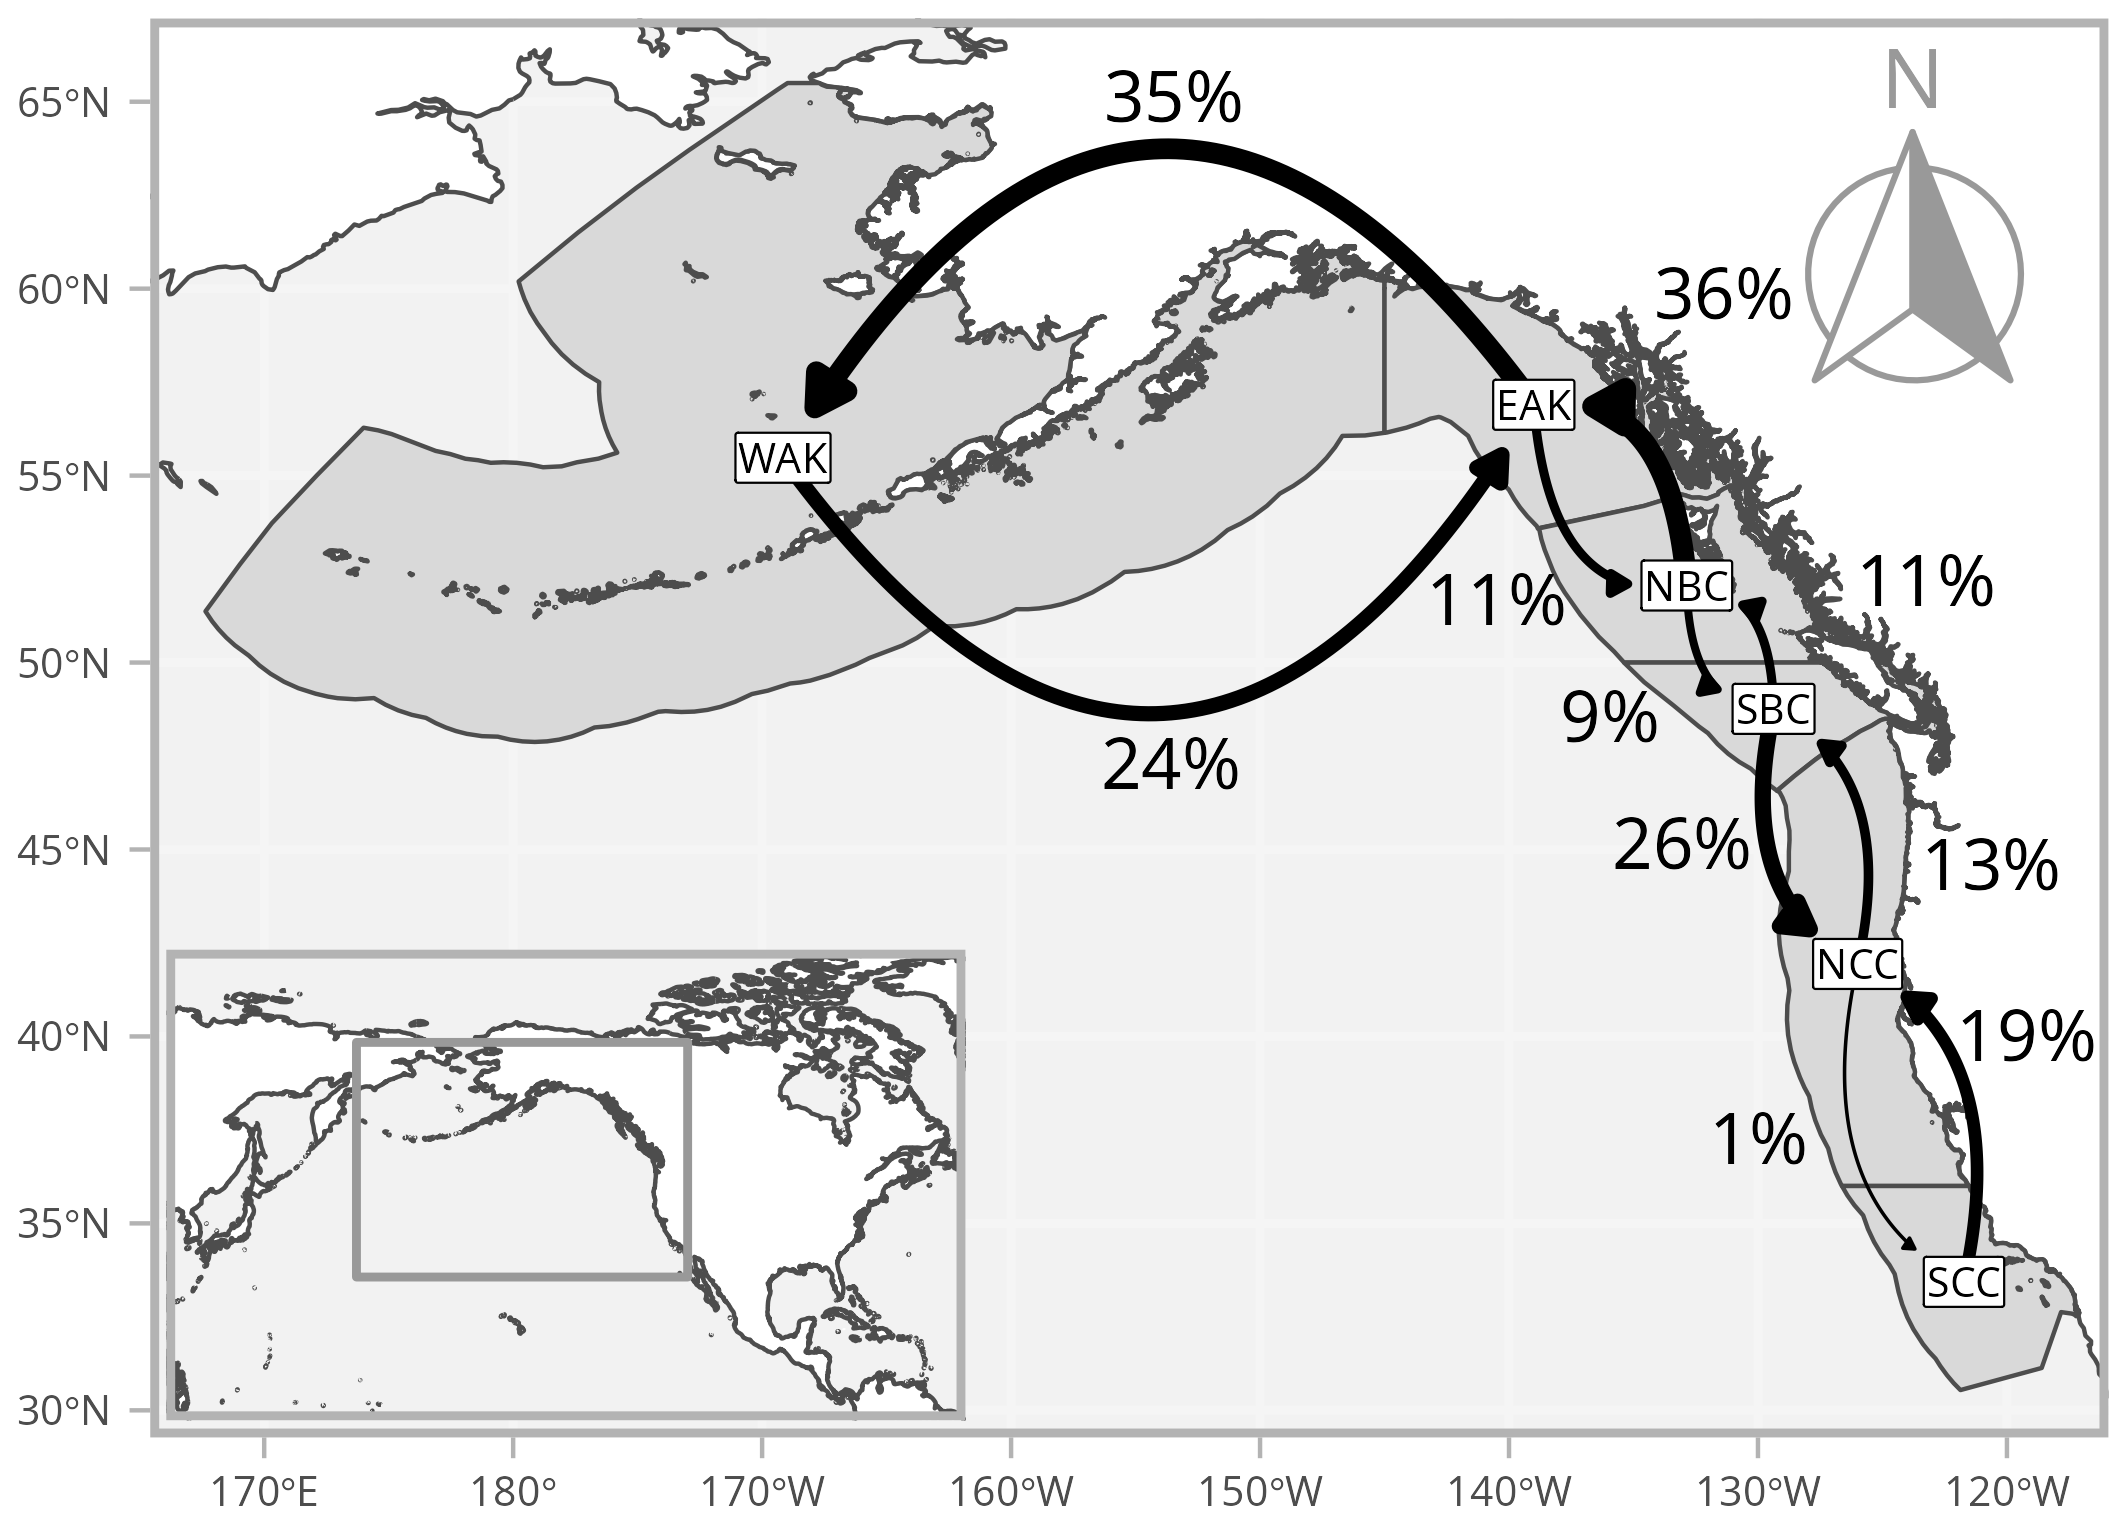
\includegraphics[width = 0.7\textwidth]{map-regions-6-network}
    \caption{TBD}
    \label{fig:map-network-regions-6}
\end{figure}

% \begin{figure}[htb]
%     \centering
%     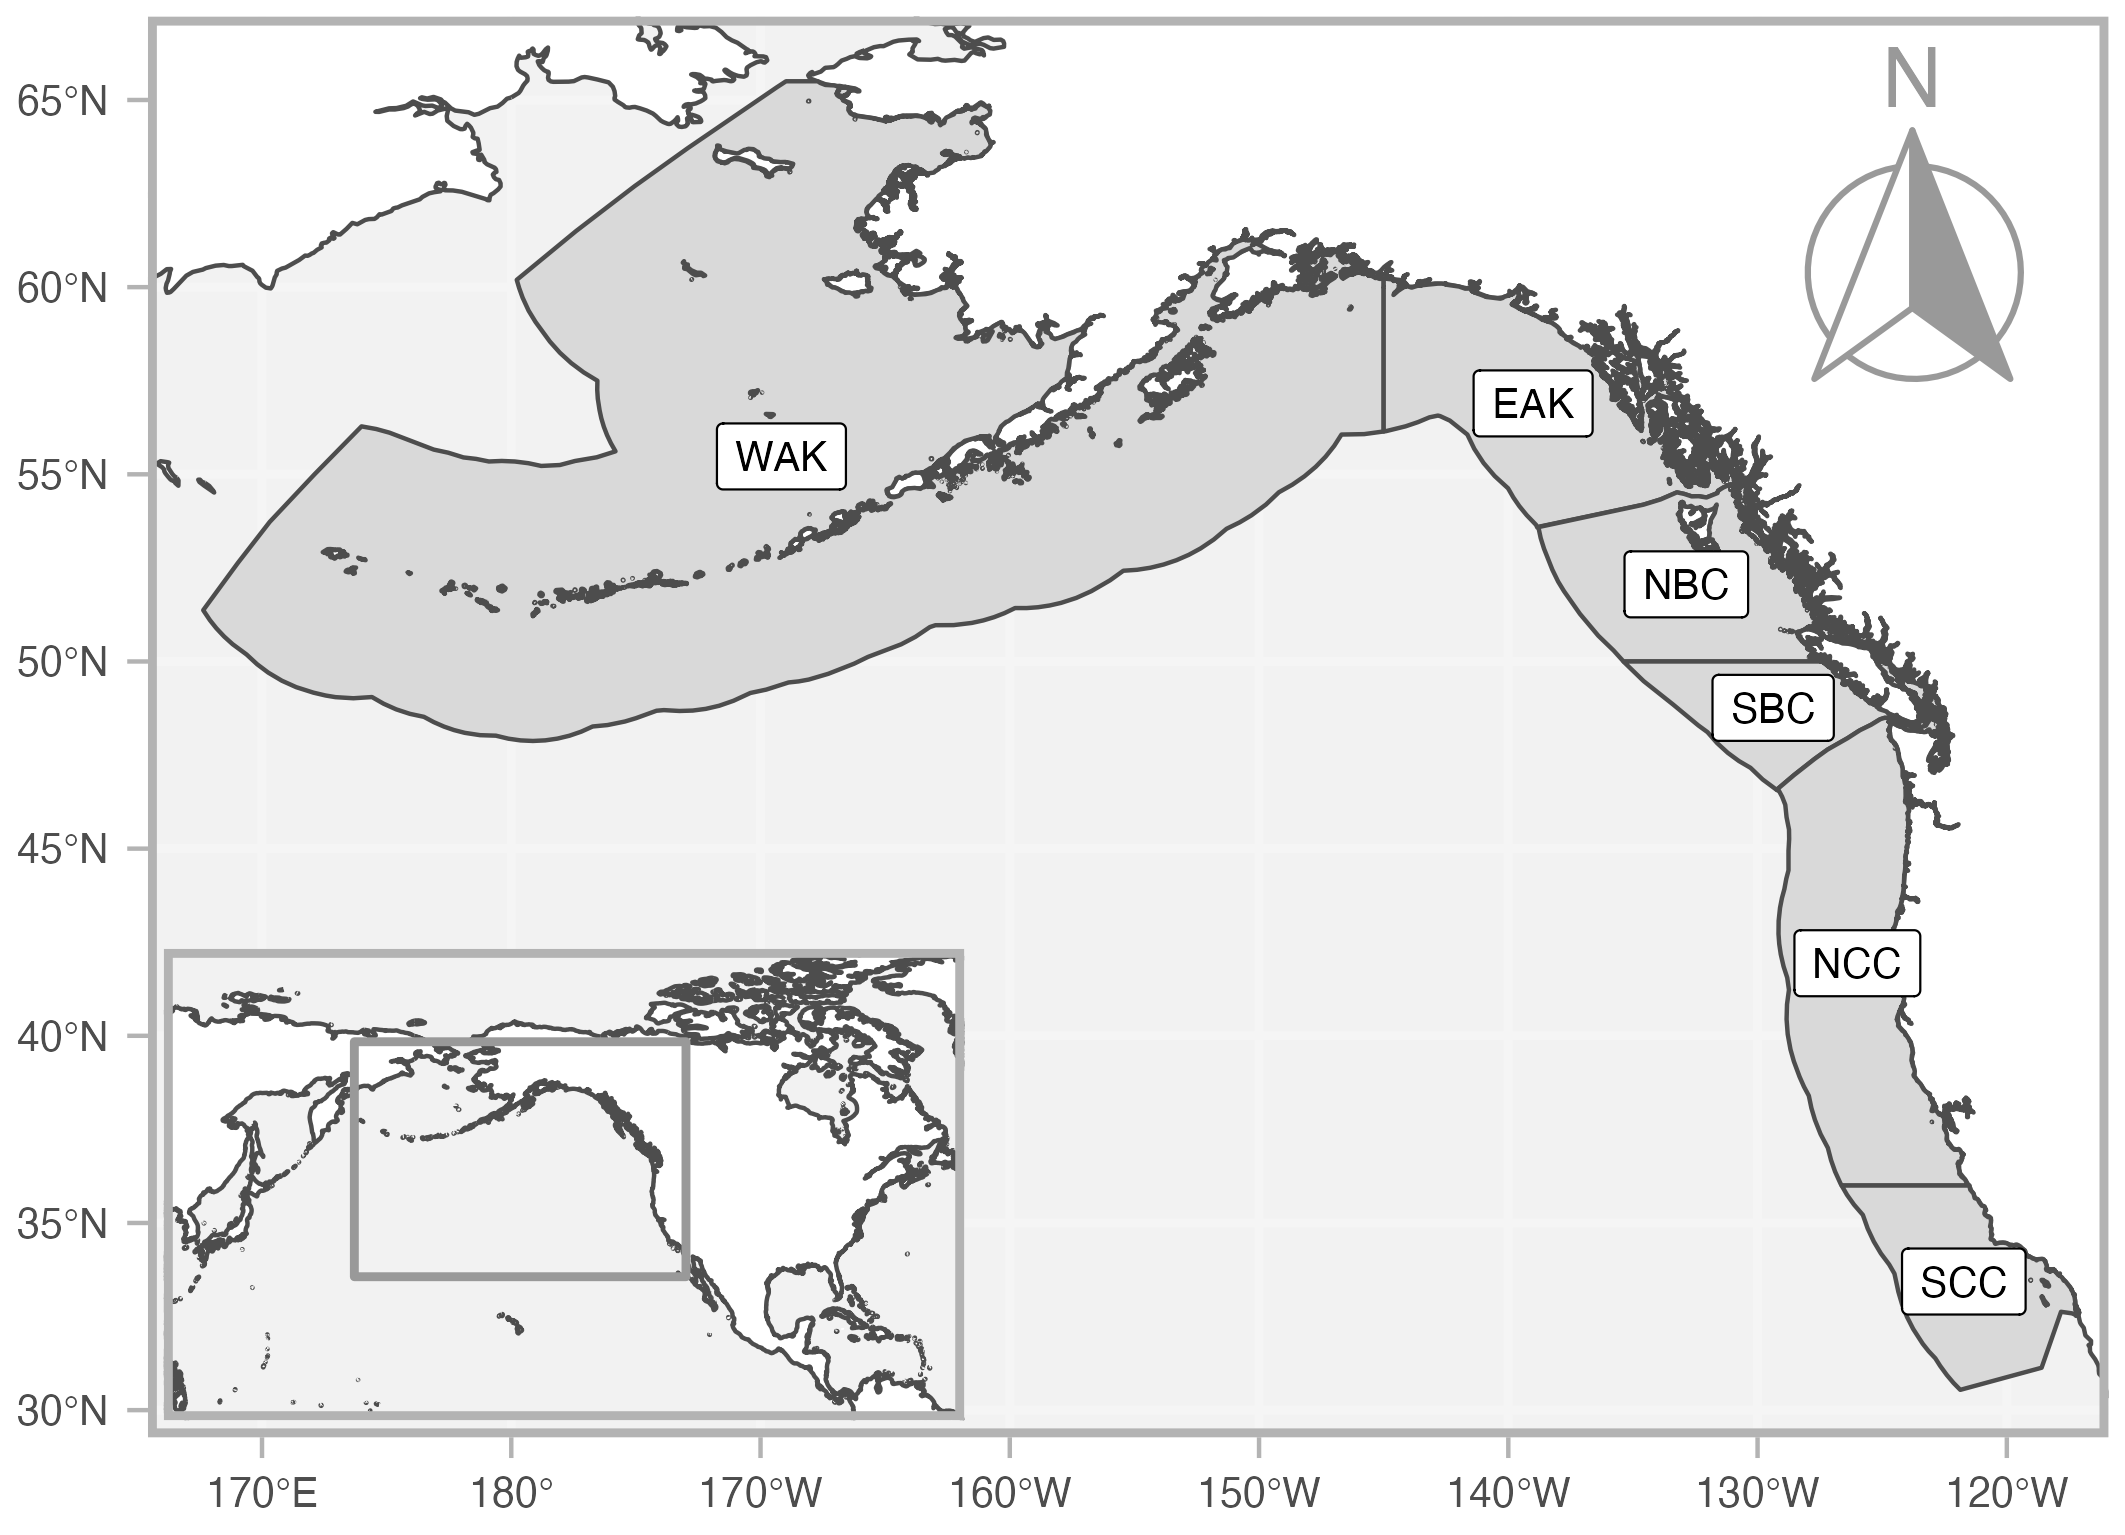
\includegraphics[width = 0.7\textwidth]{map-regions-6}
%     \caption{TBD}
%     \label{fig:map-regions-6}
% \end{figure}

\begin{figure}[htb]
    \centering
    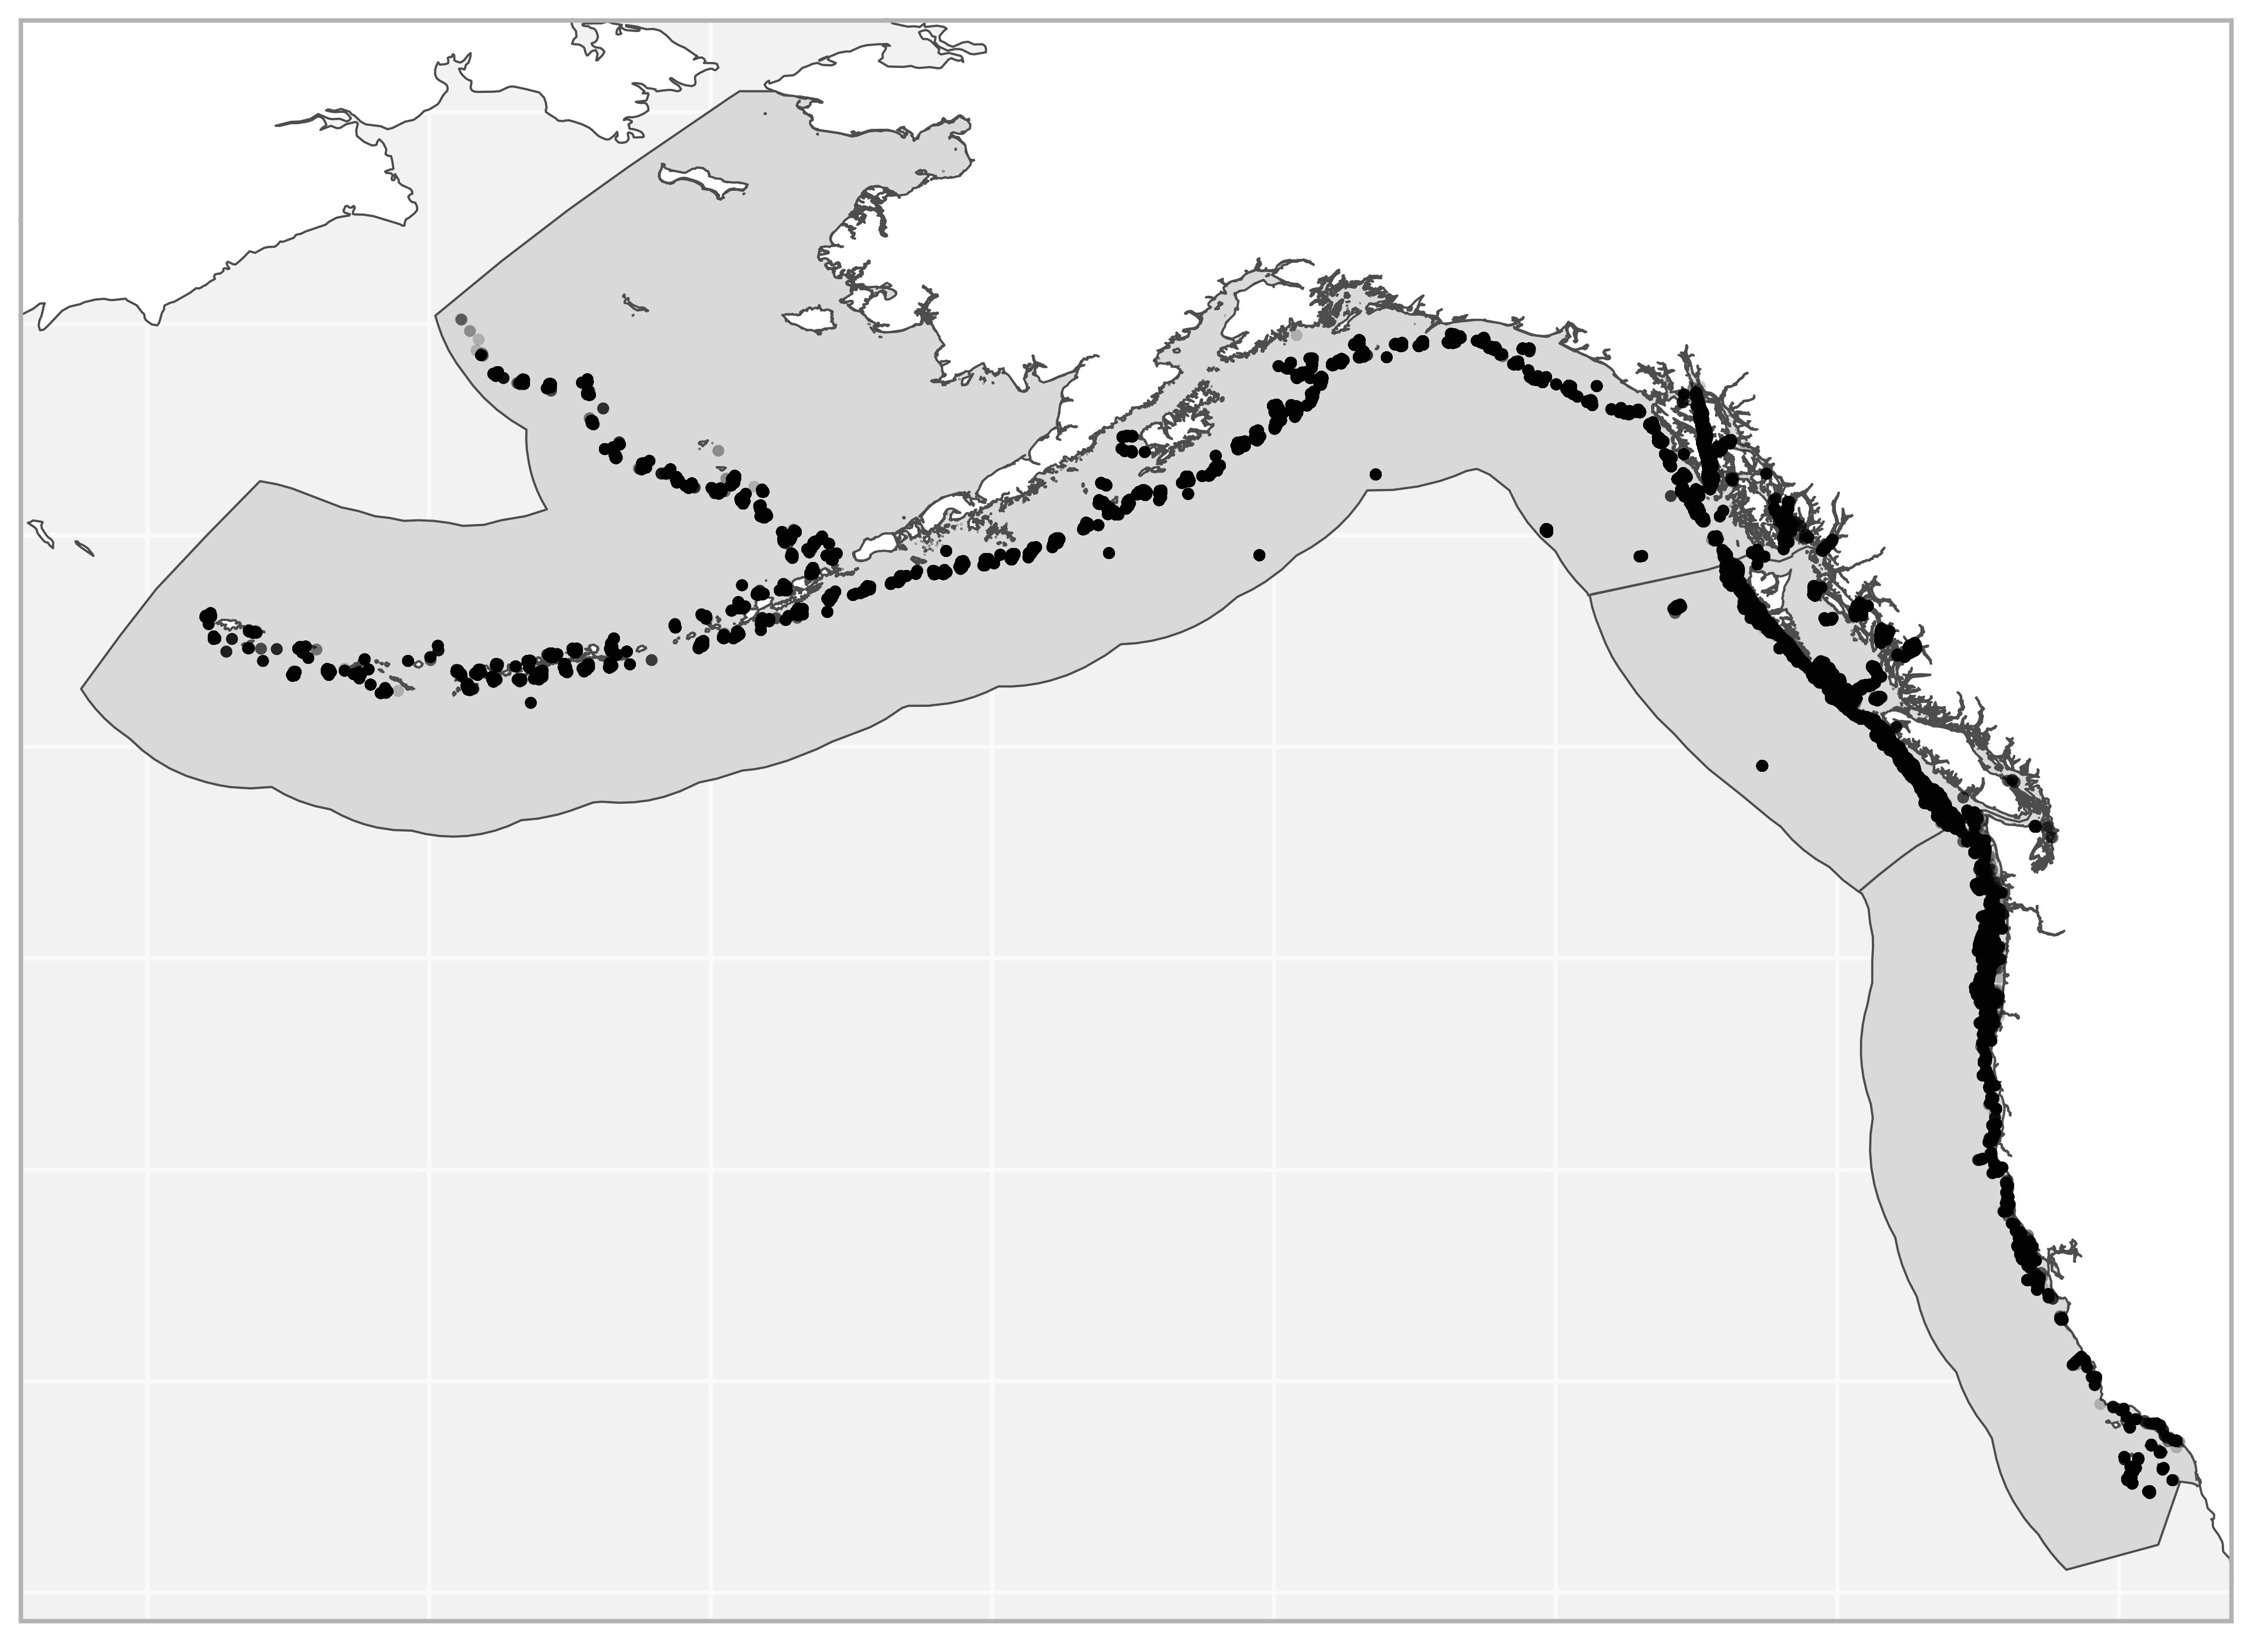
\includegraphics[width = 0.7\textwidth]{map-regions-3-released}
    \caption{TBD}
    \label{fig:map-regions-3-released}
\end{figure}

\begin{figure}[htb]
    \centering
    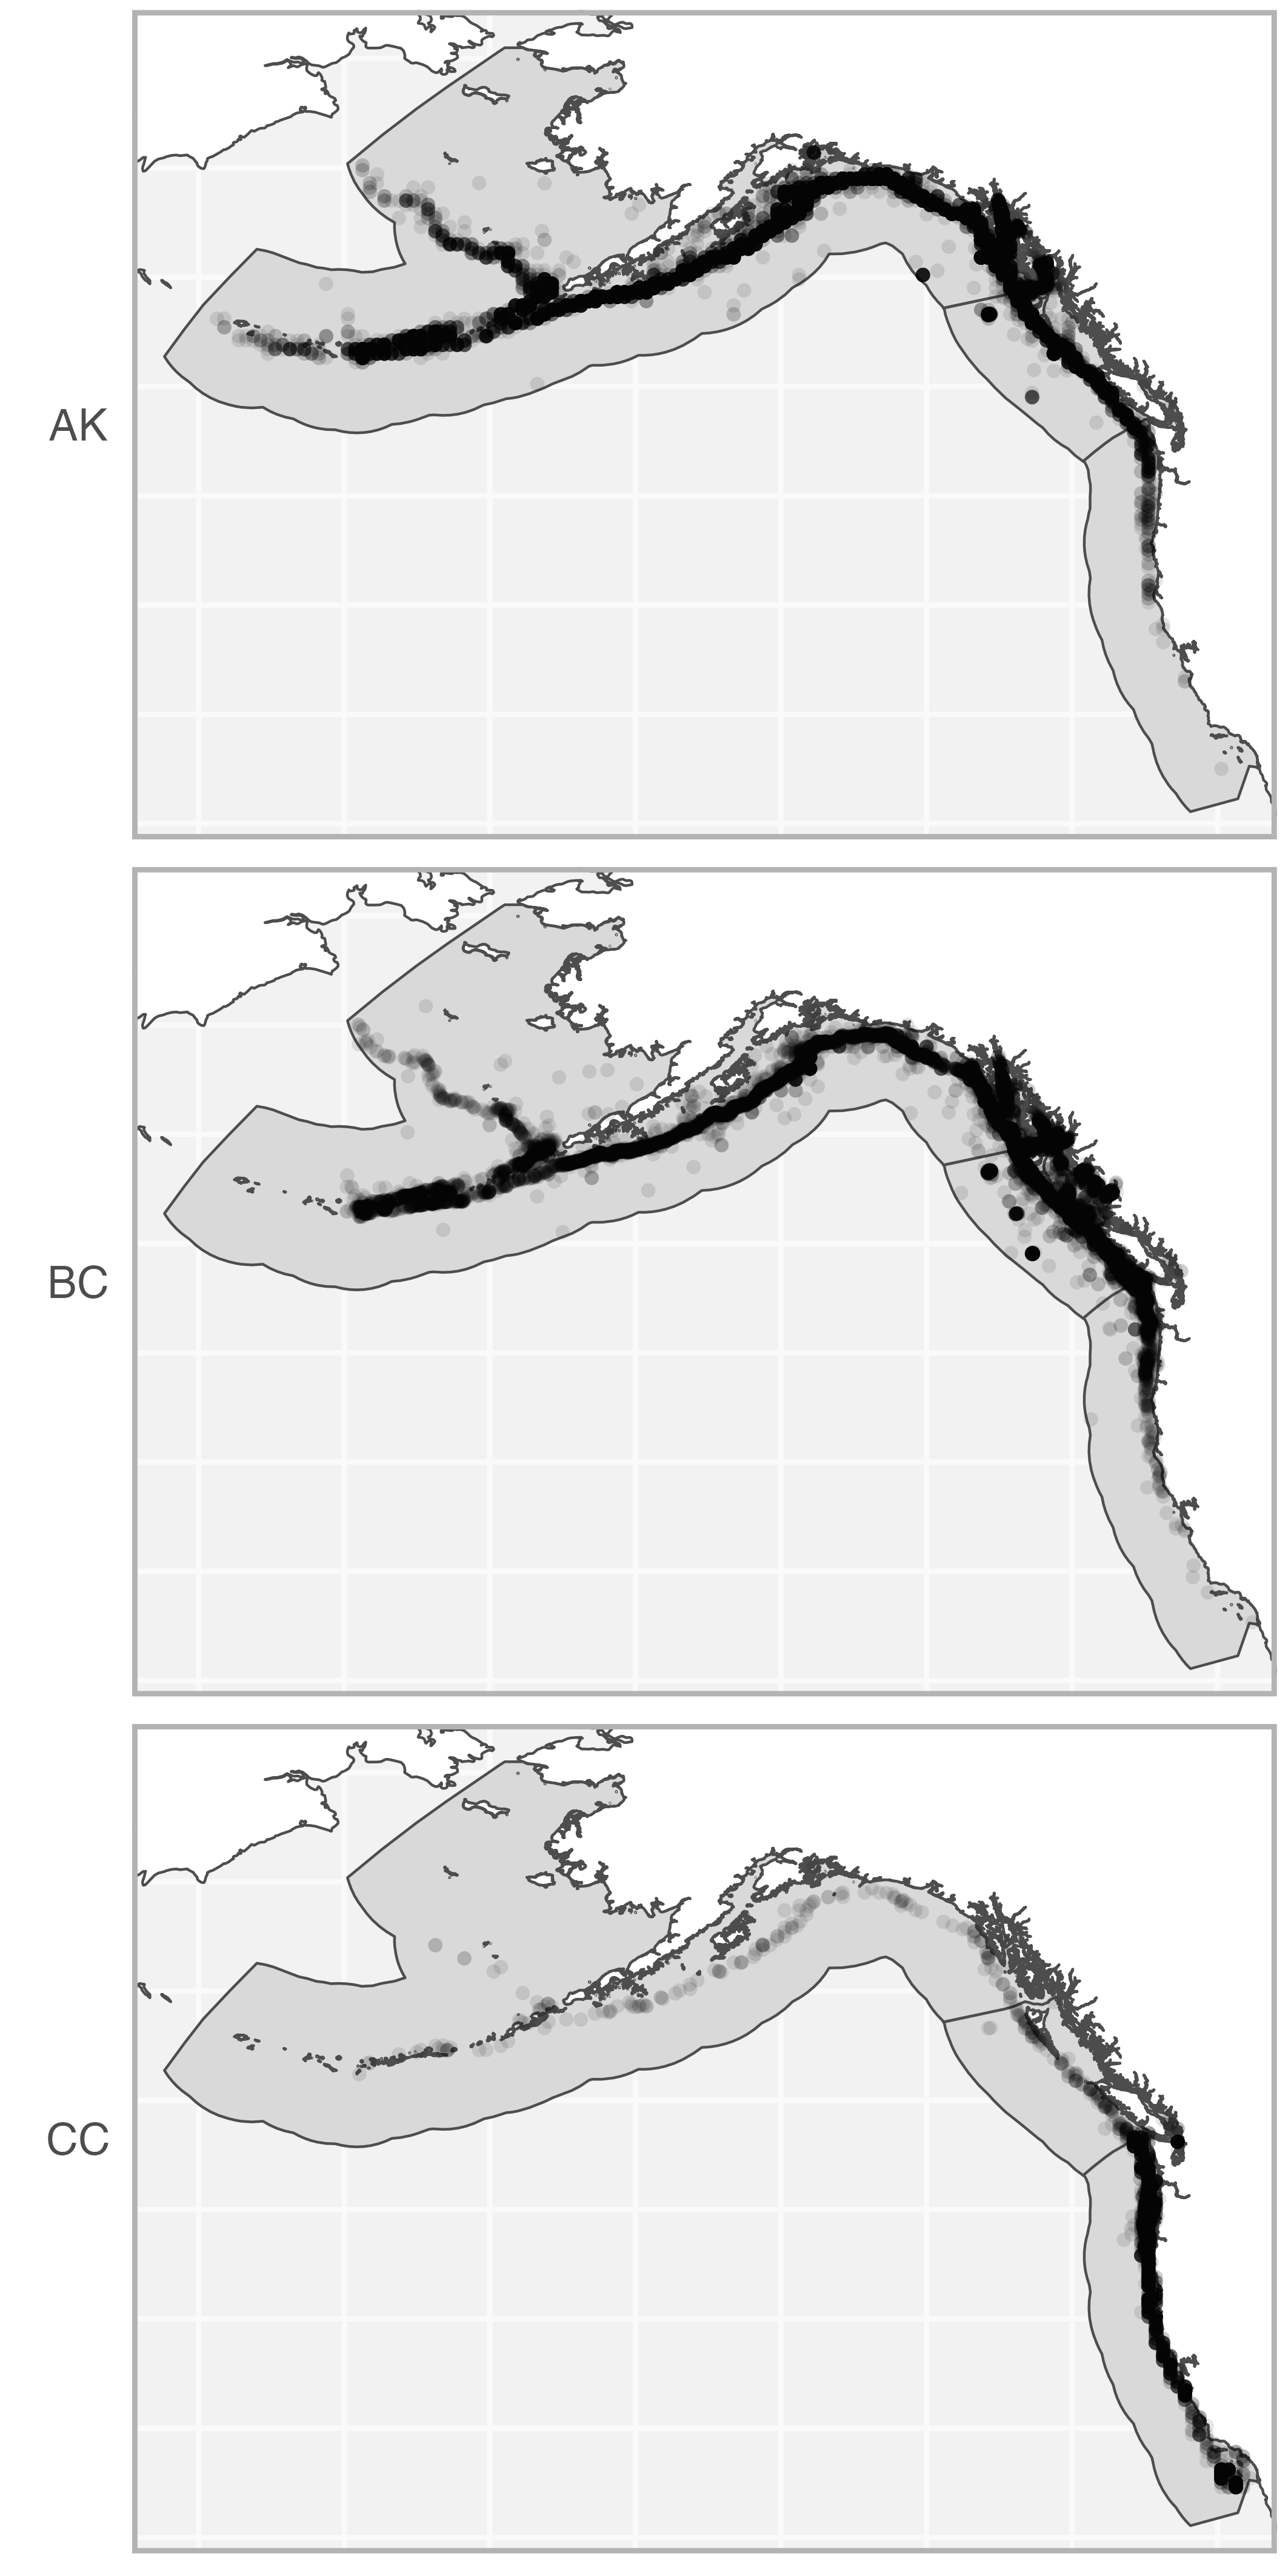
\includegraphics[width = 0.4\textwidth]{map-regions-3-recovered}
    \caption{TBD}
    \label{fig:map-regions-3-recovered}
\end{figure}

\begin{figure}[htb]
    \centering
    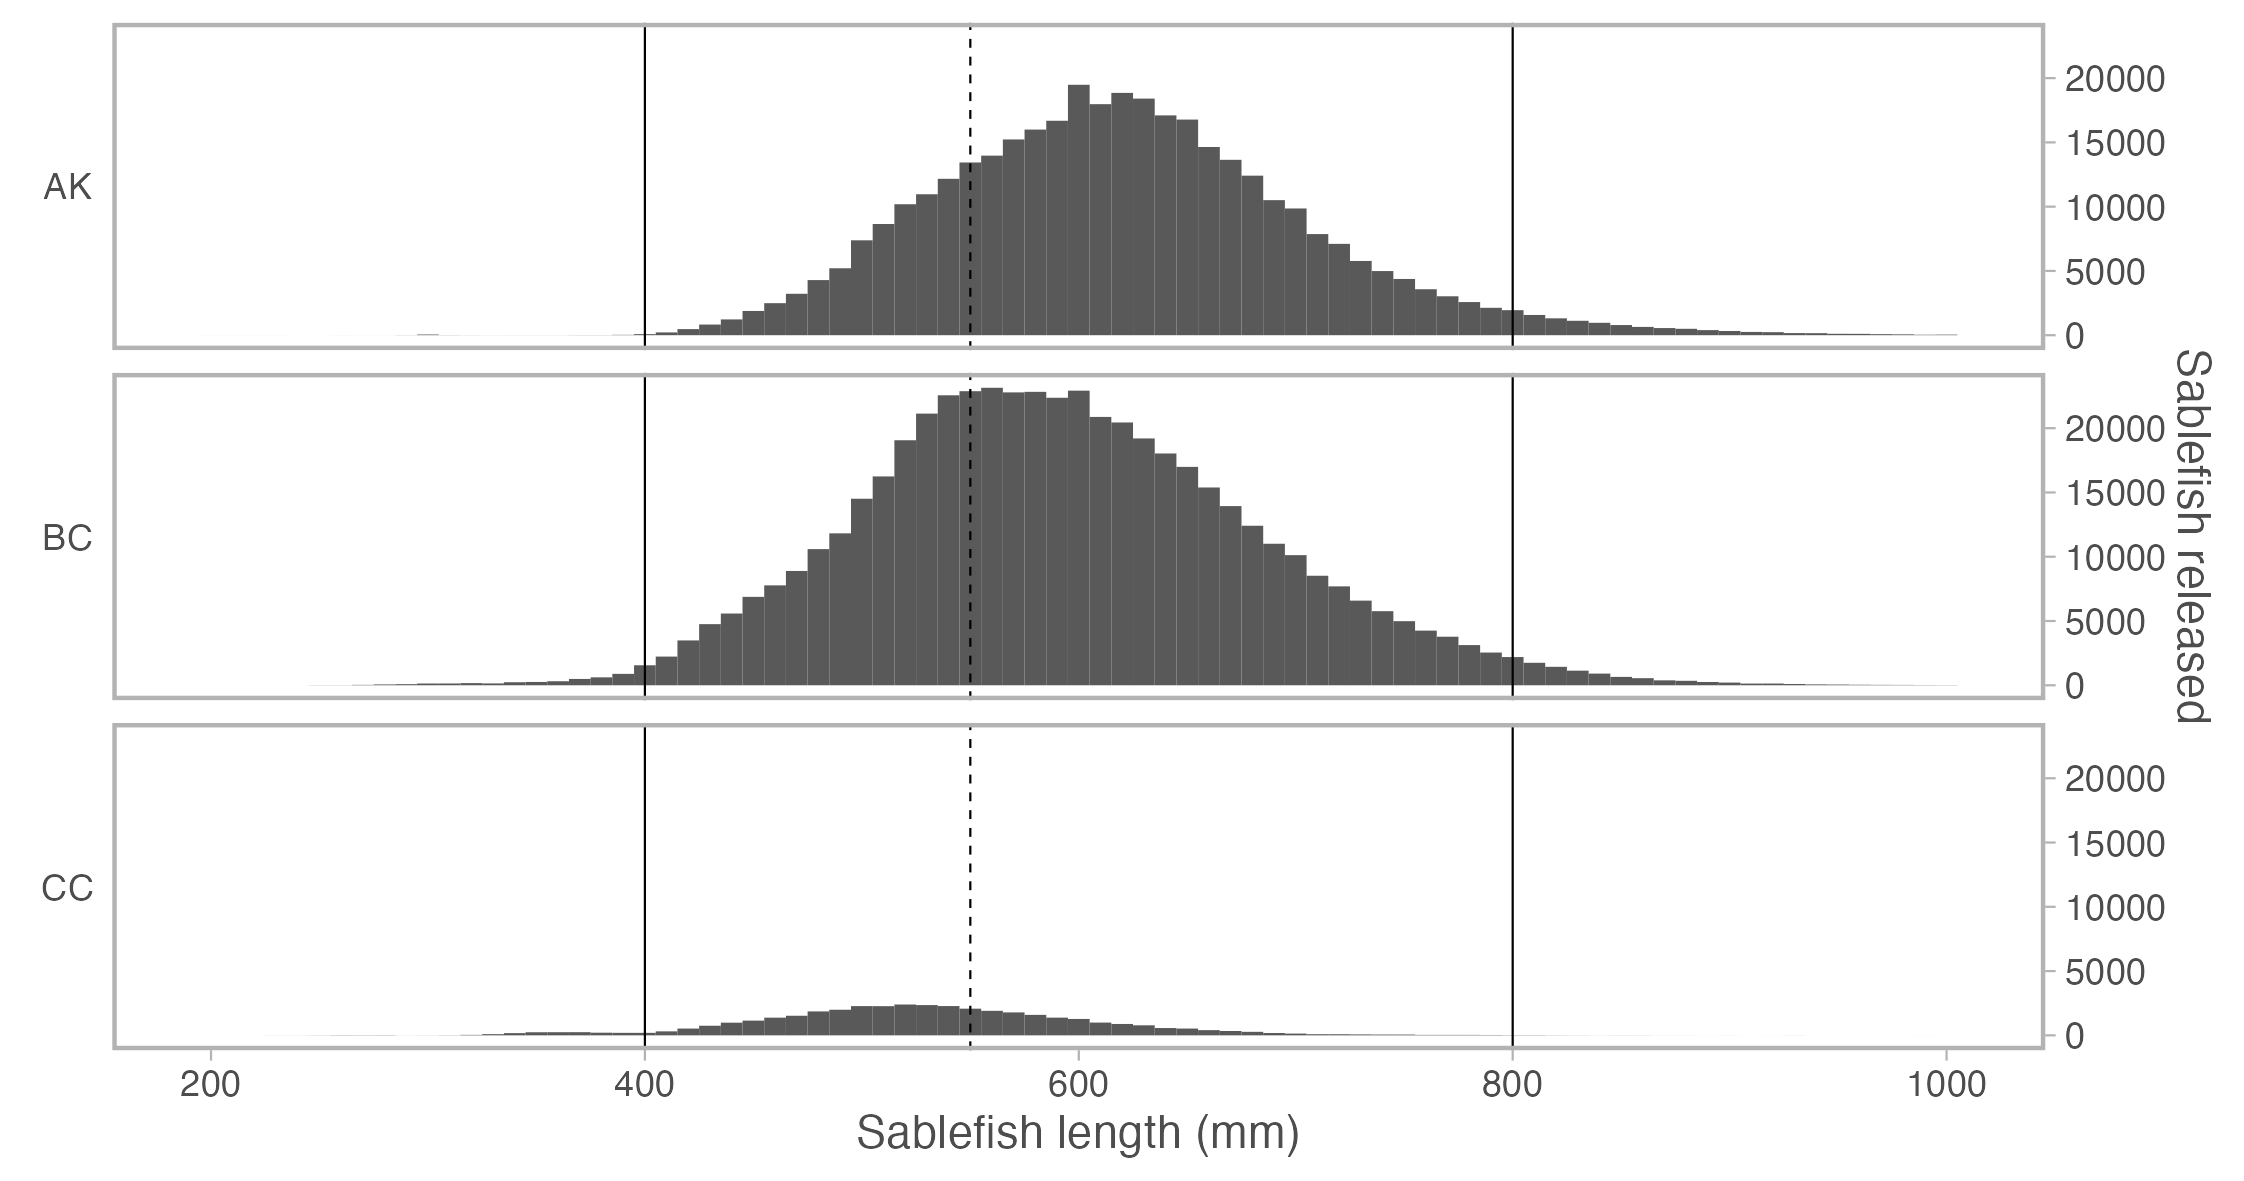
\includegraphics[width = 0.7\textwidth]{bar-regions-3-released-by-size}
    \caption{TBD}
    \label{fig:bar-regions-3-released-by-size}
\end{figure}

\begin{figure}[htb]
    \centering
    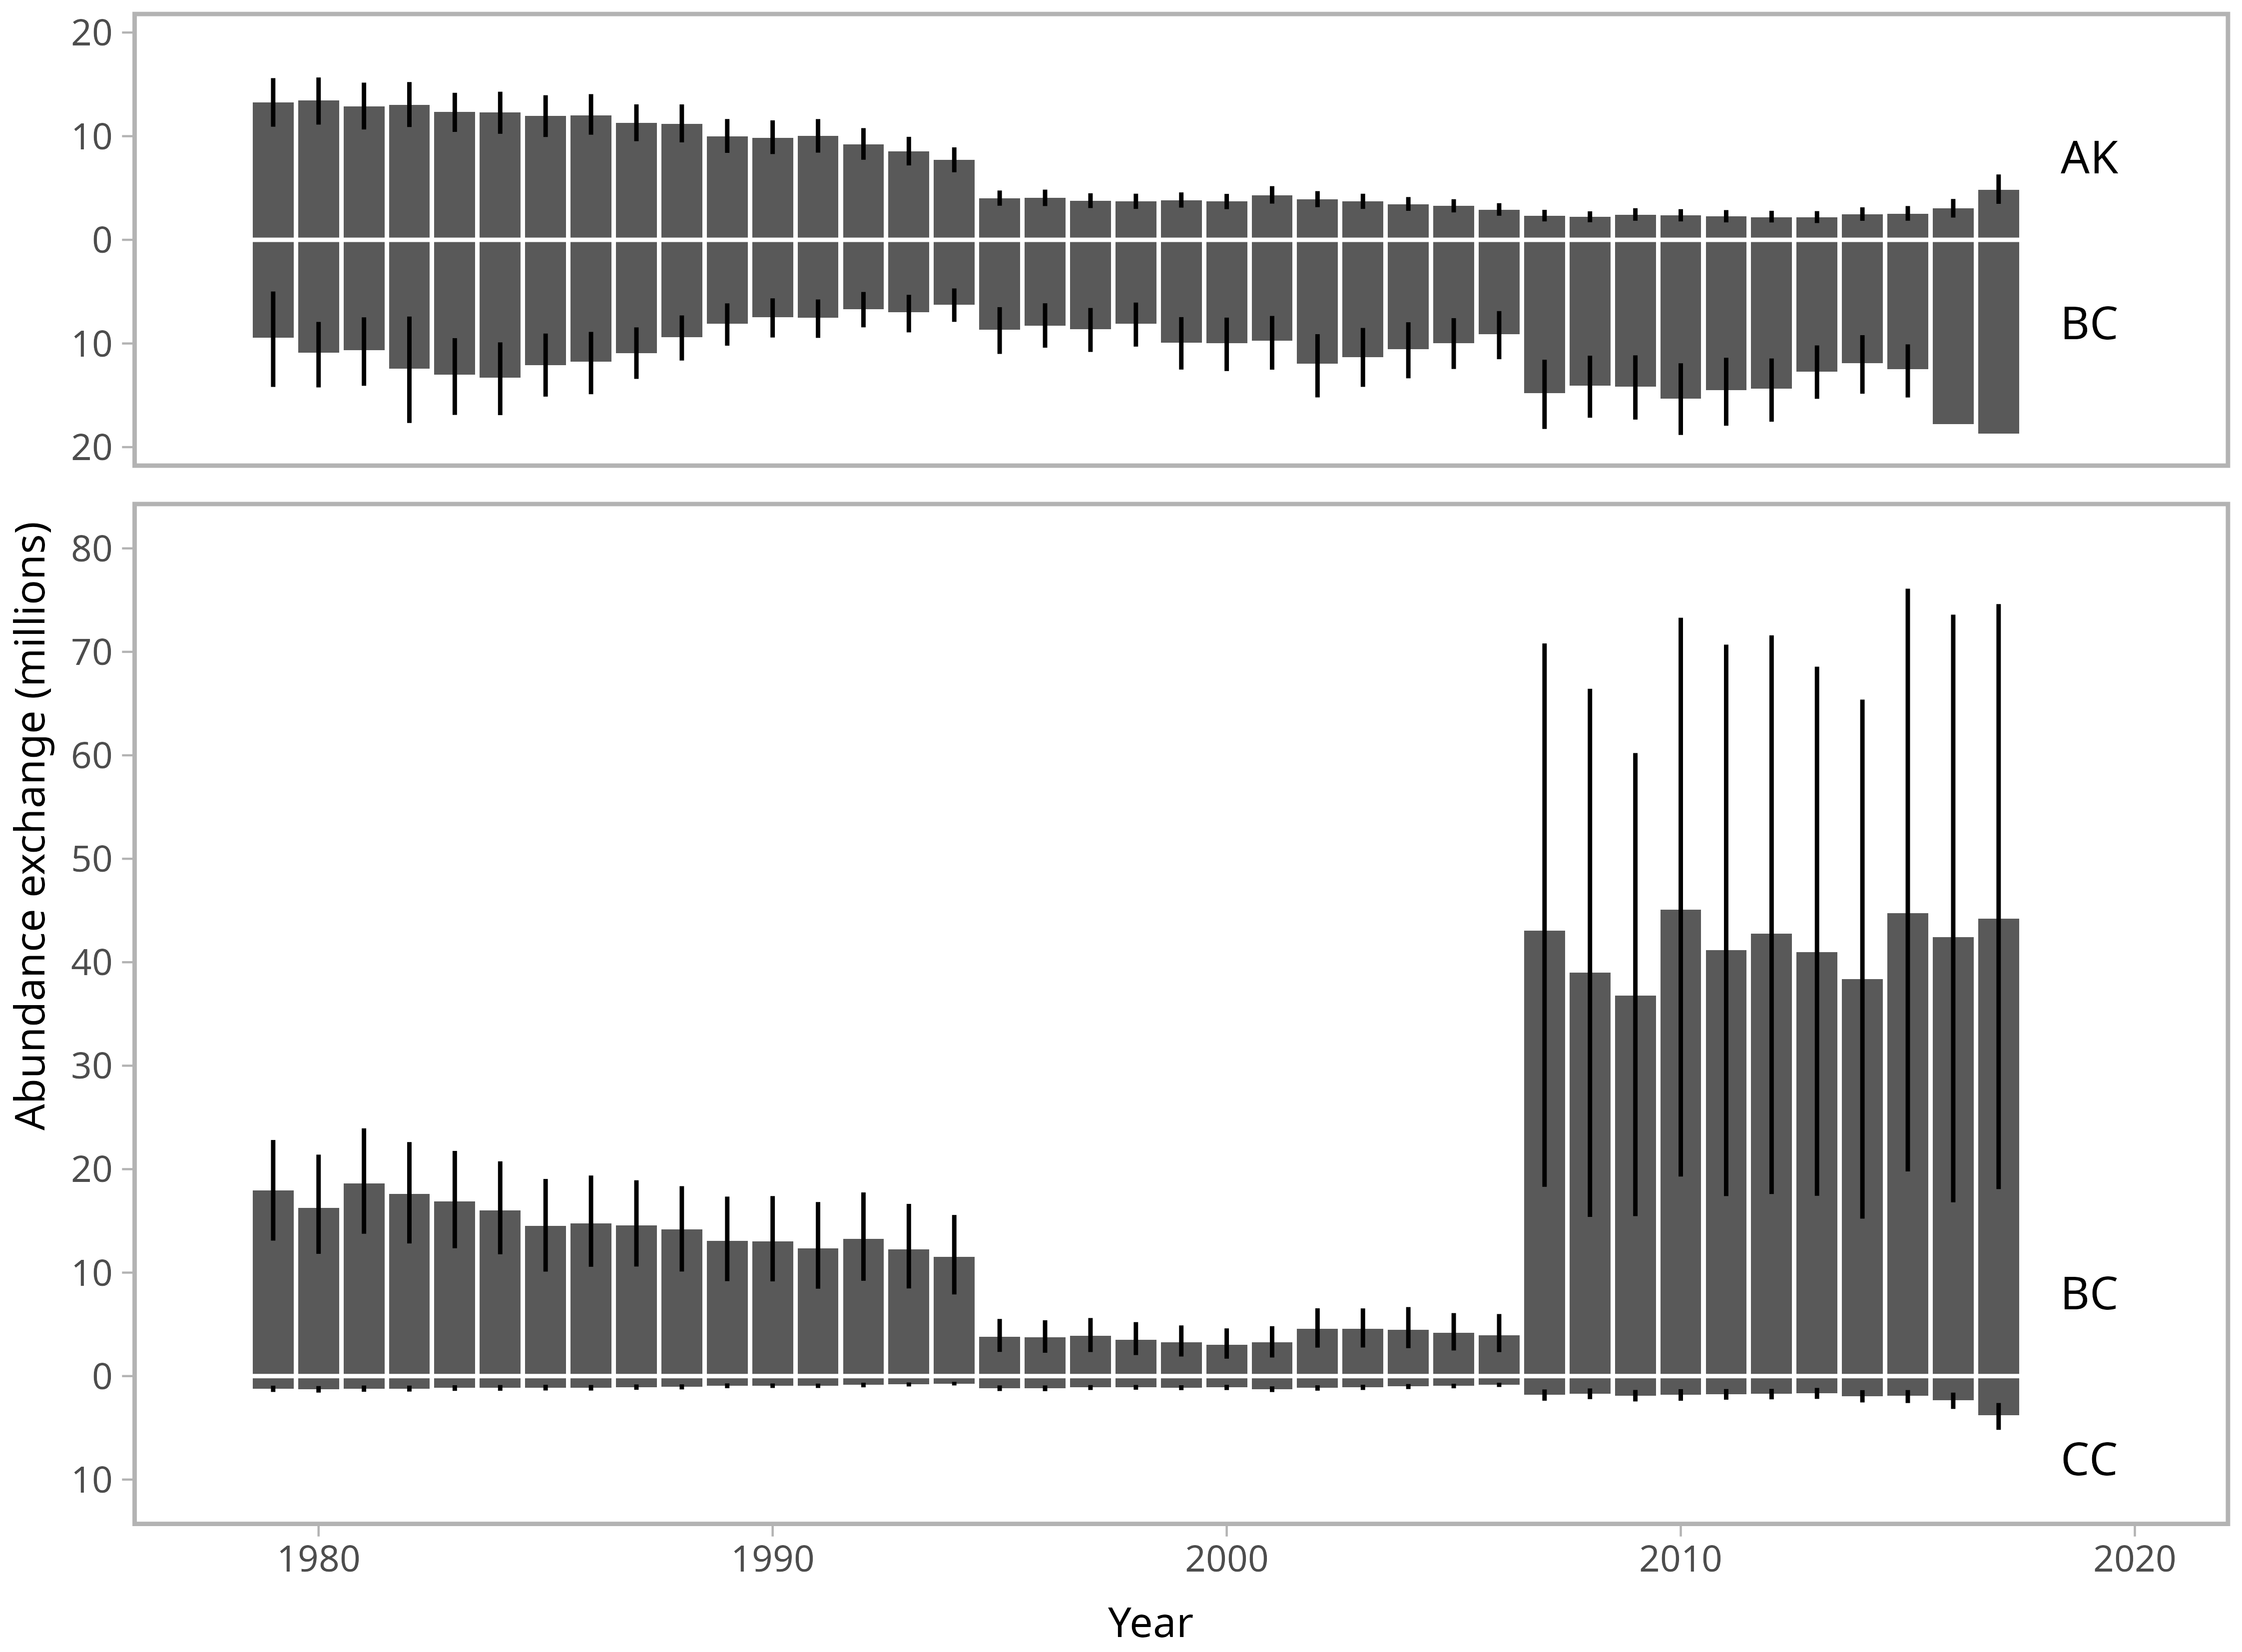
\includegraphics[width = 0.7\textwidth]{bar-abundance-exchange}
    \caption{TBD}
    \label{fig:bar-abundance-exchange}
\end{figure}

\begin{figure}[htb]
    \centering
    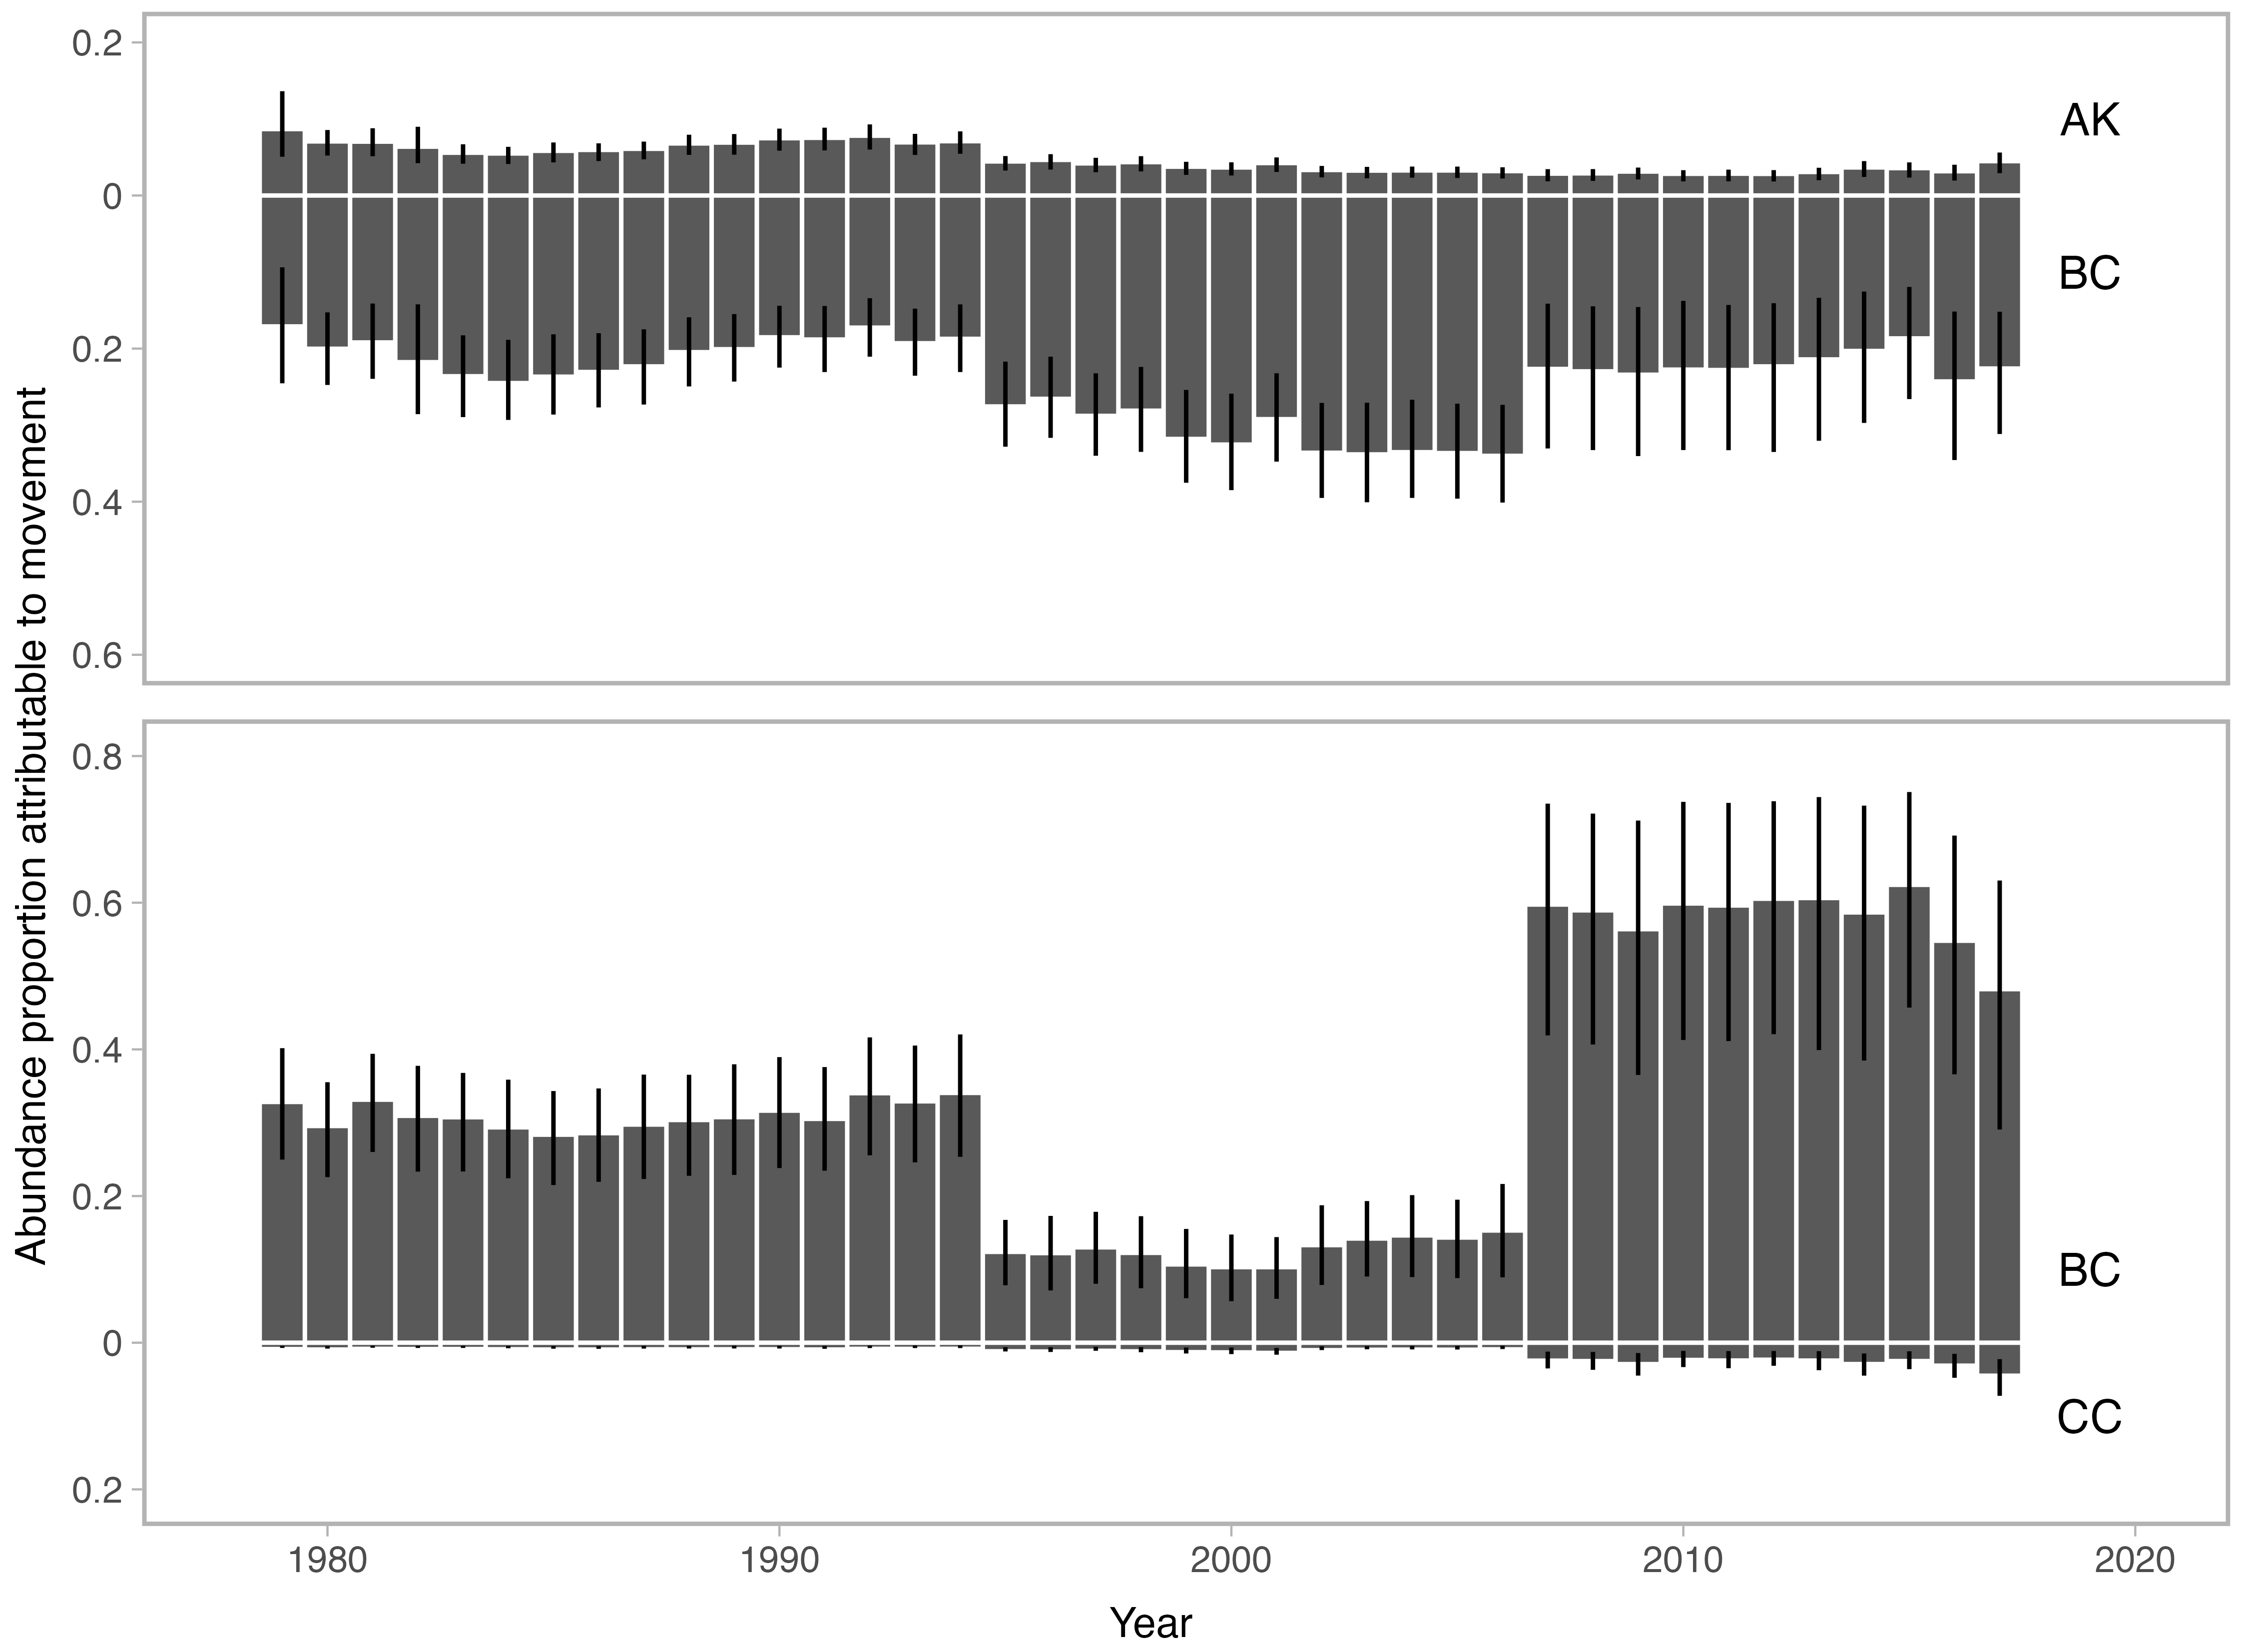
\includegraphics[width = 0.7\textwidth]{bar-percent-attributable}
    \caption{TBD}
    \label{fig:bar-percent-attributable}
\end{figure}

\section{Tables}


\begin{table}[h]
  \begin{center}
  \caption{Sablefish movement rates between regions (per fish per year).}
  \label{tab:movement-rate-regions-6-mean}
    \pgfplotstabletypeset[
      col sep=comma,                       % Commas separate .csv values
      columns/{0}/.style={column name={}}, % Replace autofilled column name by " "
      string type                          % Expect characters
    ]{tabs/movement-rate-regions-6-mean.csv}
  \end{center}
\end{table}

\section{Supplementary information}

% Example table script
\begin{table}[h]
  \begin{center}
  \caption{Sablefish movement rates between regions (per fish per year).}
  \label{tab:movement-rate-regions-3-mean}
    \pgfplotstabletypeset[
      col sep=comma,                       % Commas separate .csv values
      columns/{0}/.style={column name={}}, % Replace autofilled column name by " "
      string type                          % Expect characters
    ]{tabs/movement-rate-regions-3-mean.csv}
  \end{center}
\end{table}

\begin{figure}[htb]
    \centering
    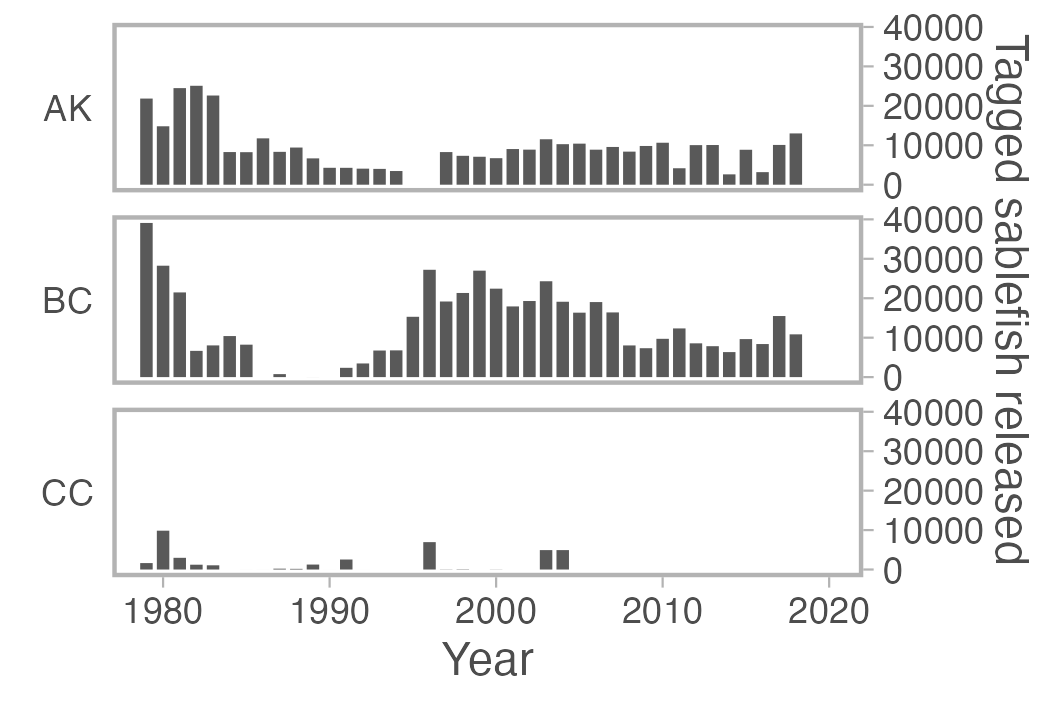
\includegraphics[width = 0.7\textwidth]{bar-regions-3-released-by-year}
    \caption{TBD}
    \label{fig:bar-regions-3-released-by-year}
\end{figure}

\begin{figure}[htb]
    \centering
    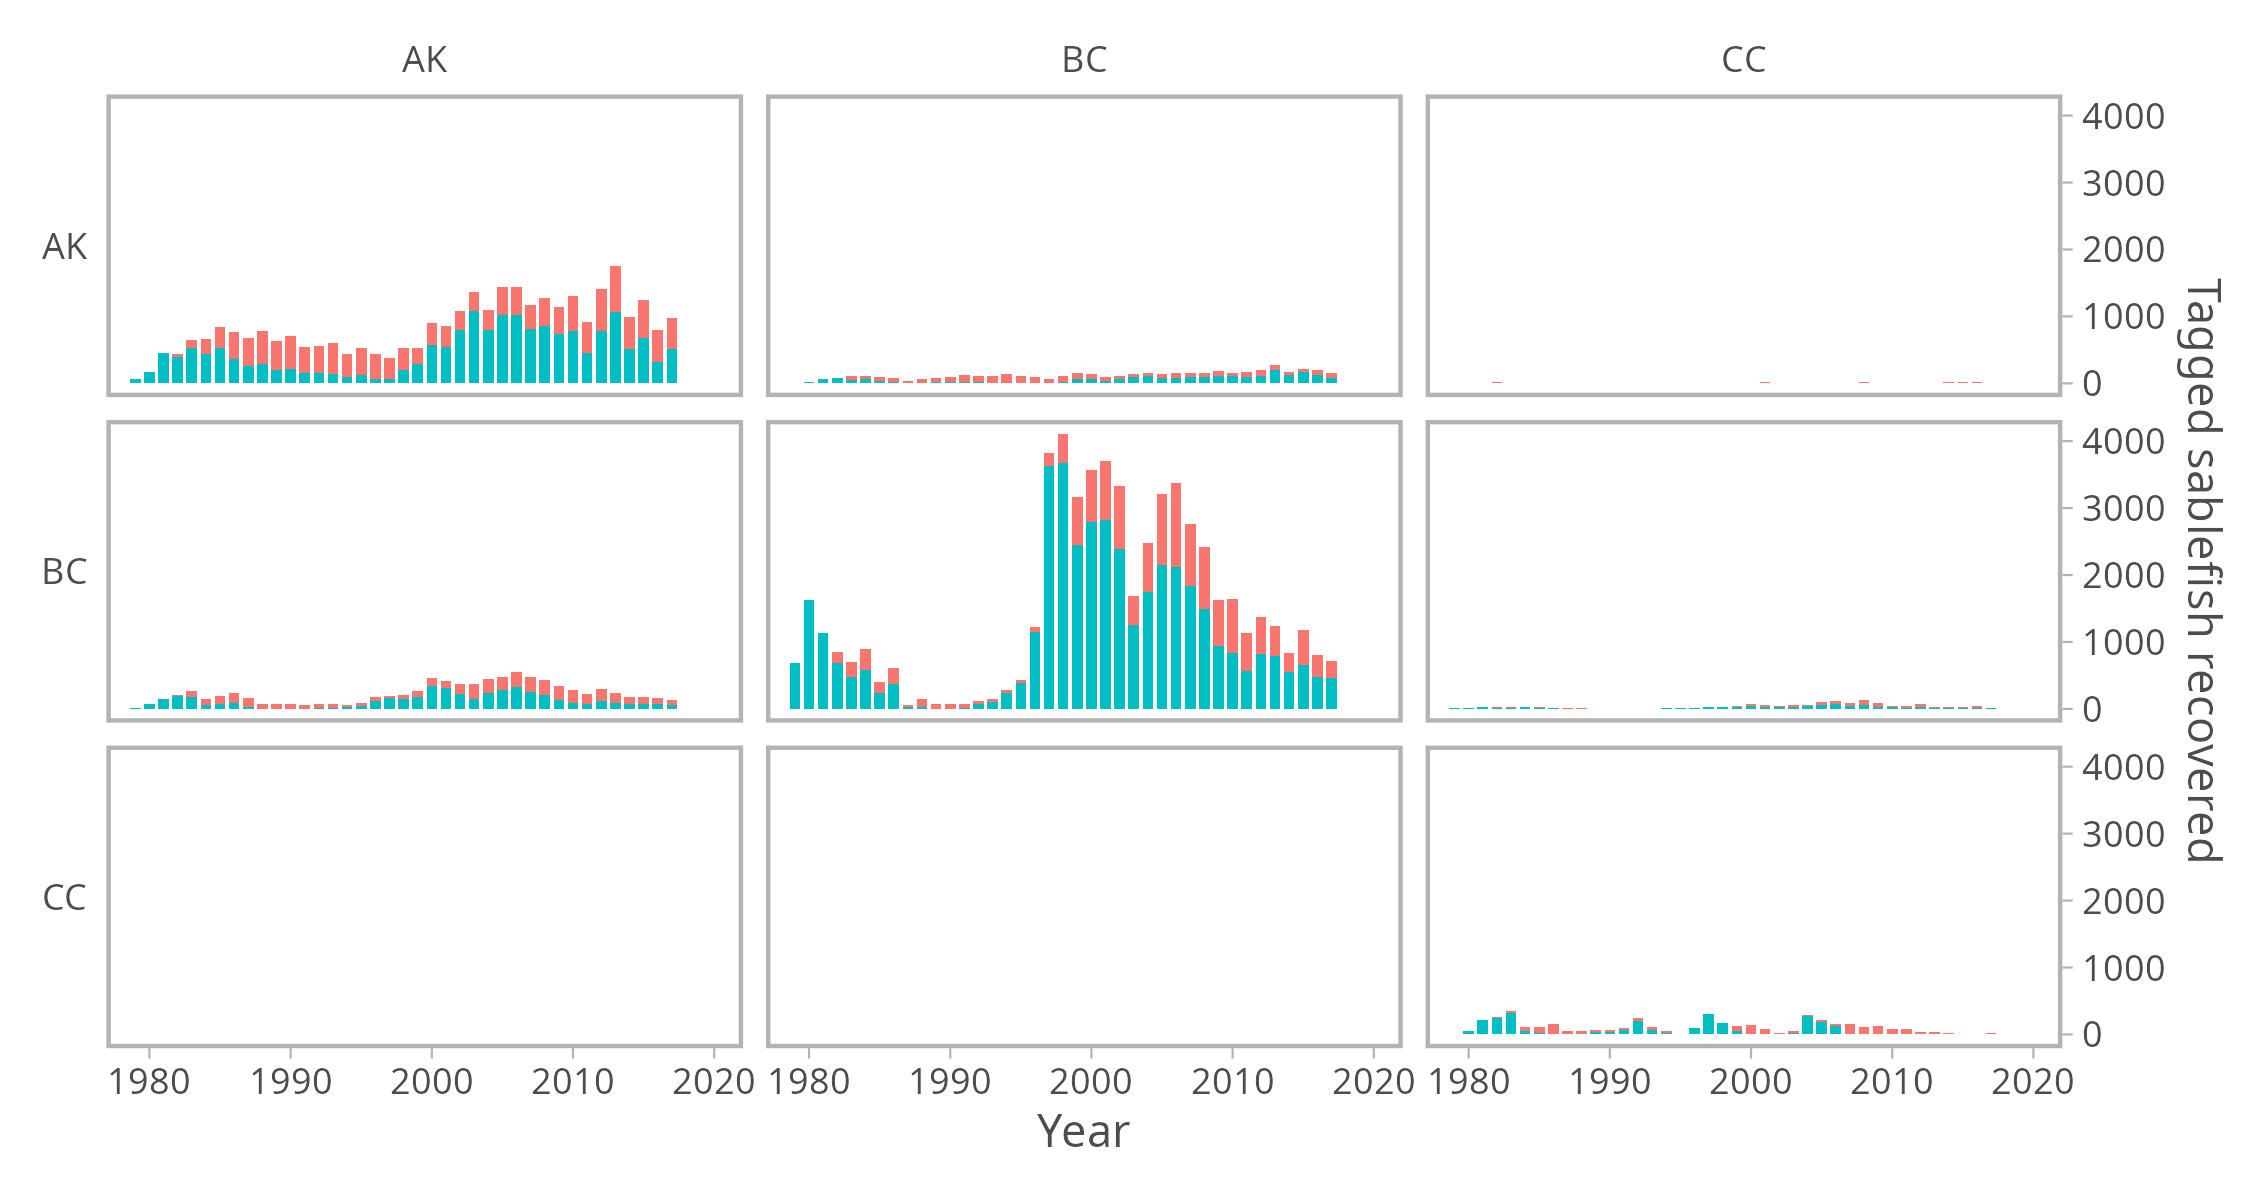
\includegraphics[width = 0.7\textwidth]{bar-regions-3-recovered-by-year}
    \caption{TBD}
    \label{fig:bar-regions-3-recovered-by-year}
\end{figure}

\begin{figure}[htb]
    \centering
    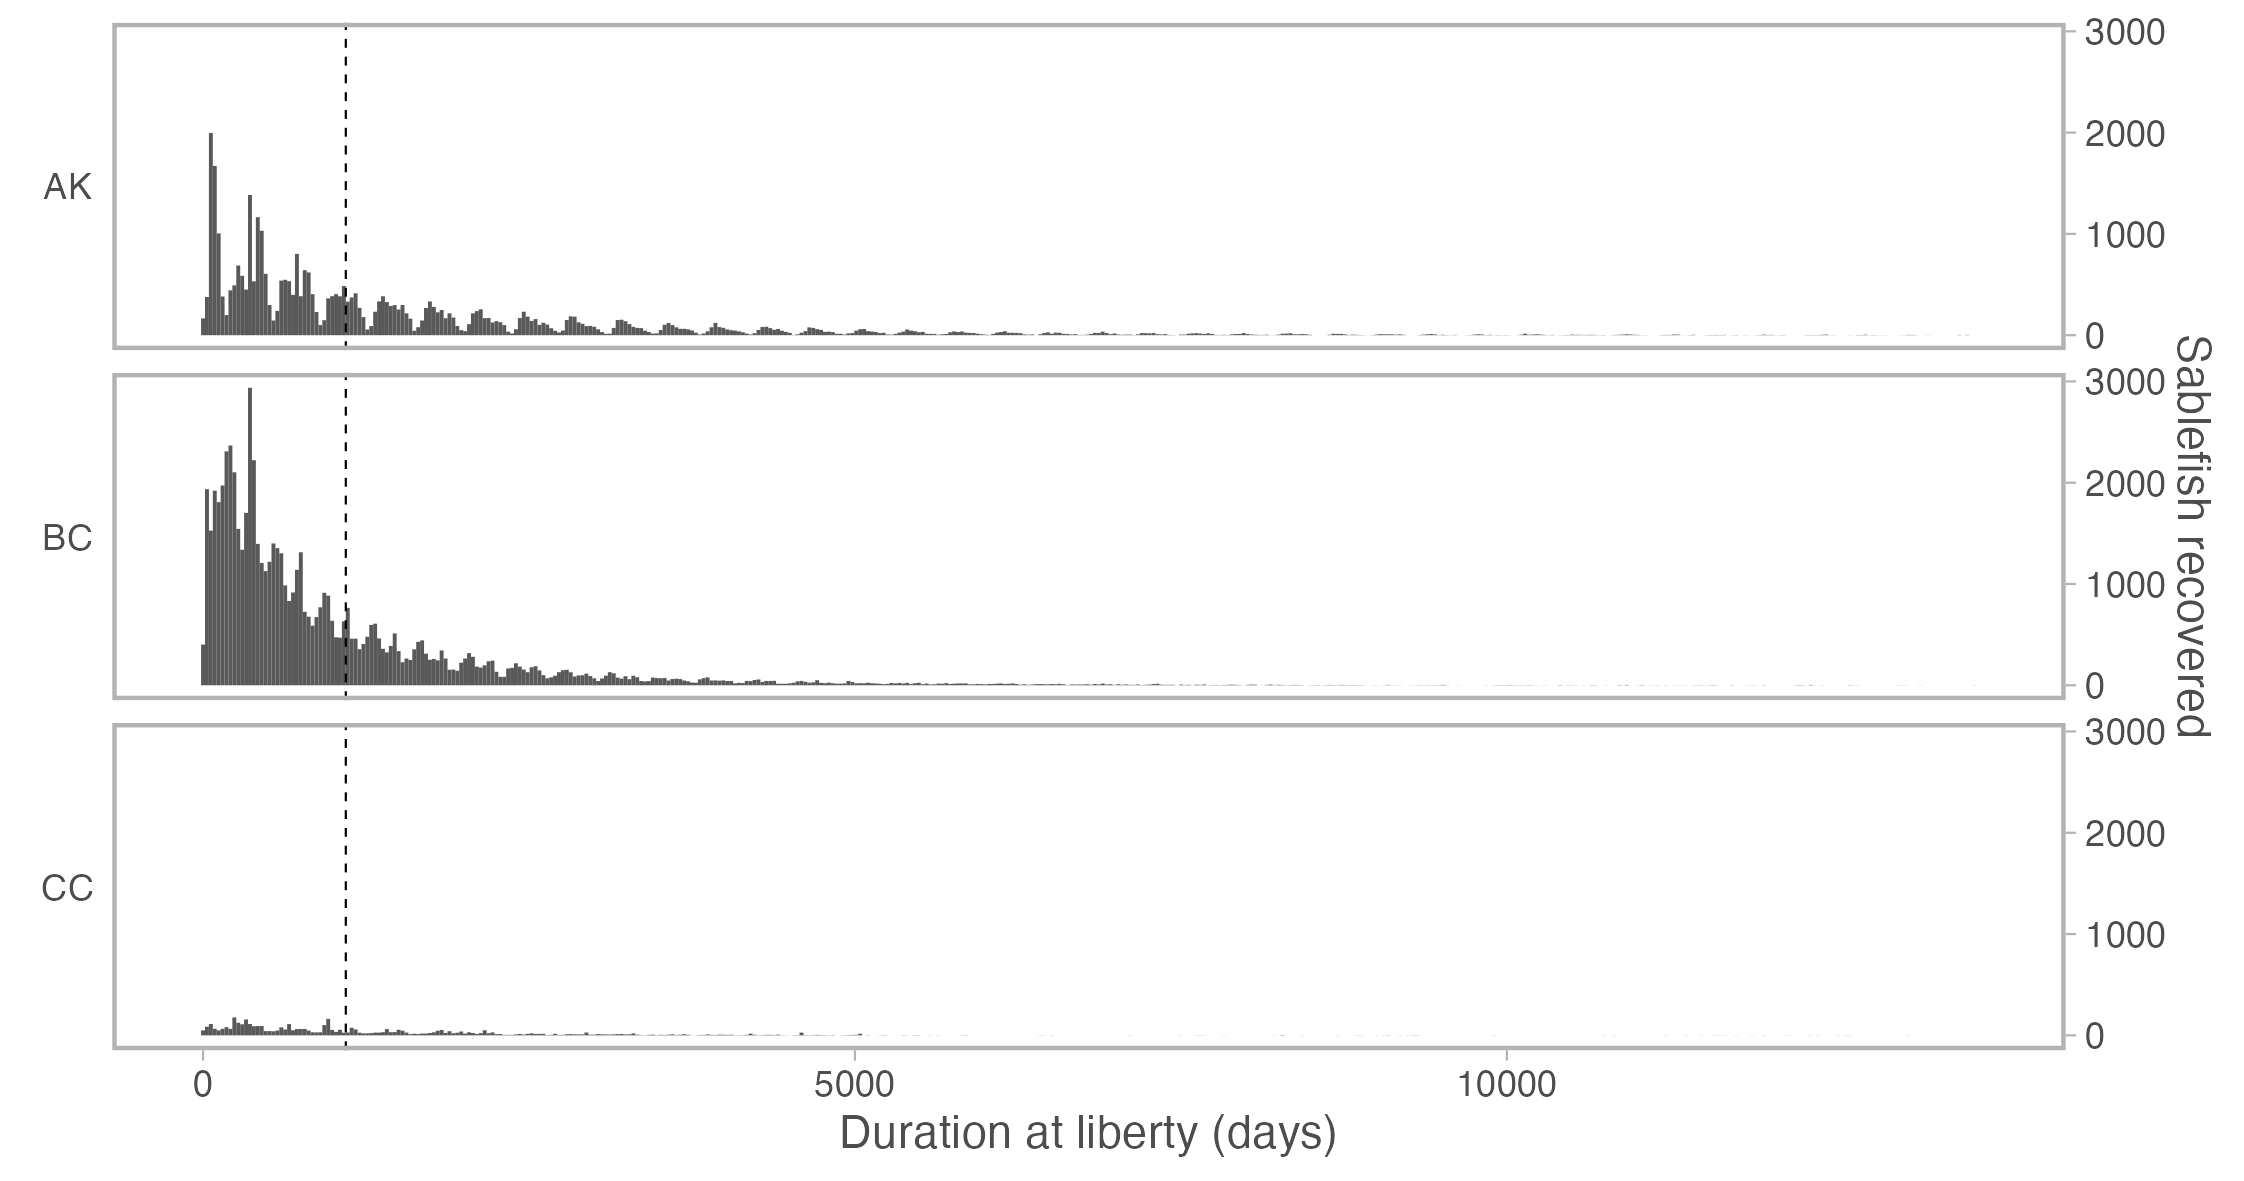
\includegraphics[width = 0.7\textwidth]{bar-regions-3-duration-at-liberty}
    \caption{TBD}
    \label{fig:bar-regions-3-duration-at-liberty}
\end{figure}

\begin{figure}[htb]
    \centering
    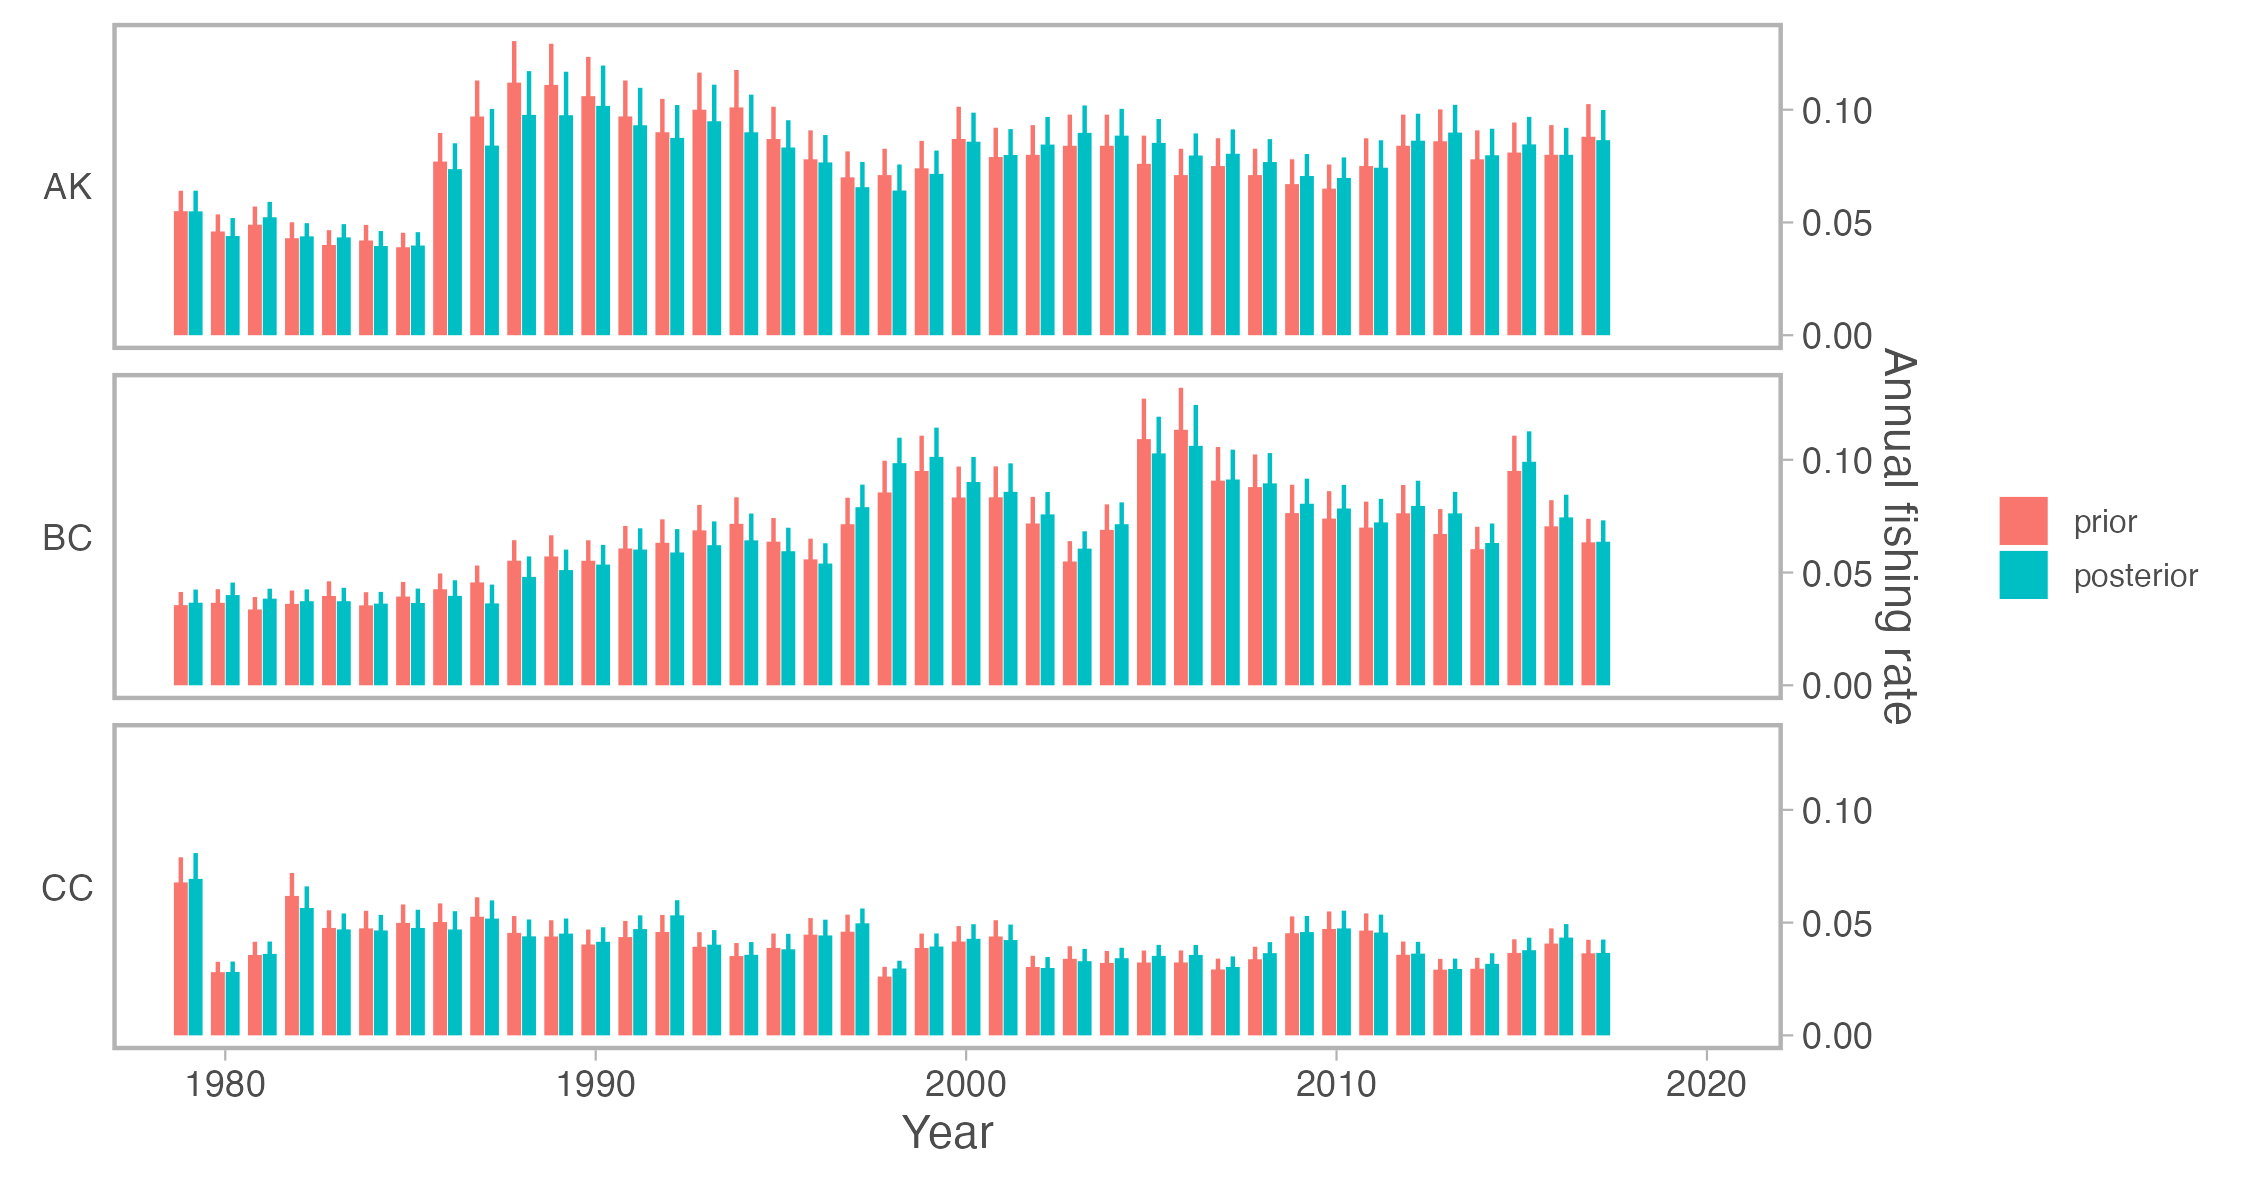
\includegraphics[width = 0.7\textwidth]{bar-regions-3-fishing-priors-posteriors}
    \caption{TBD}
    \label{fig:bar-regions-3-fishing-priors-posteriors}
\end{figure}

\begin{figure}[htb]
    \centering
    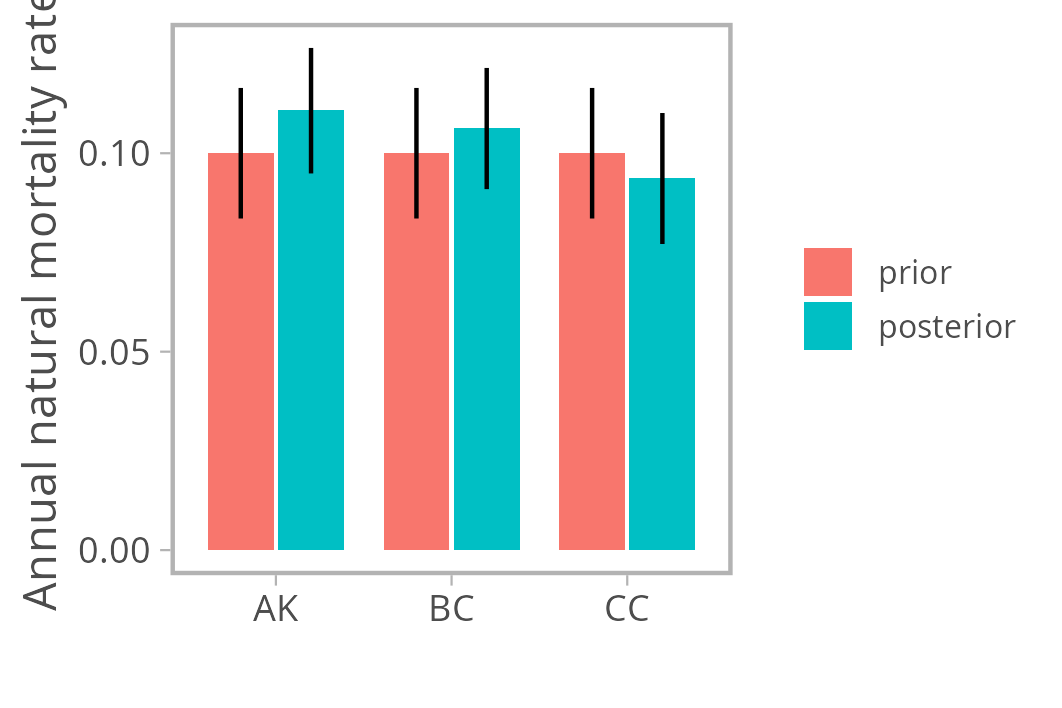
\includegraphics[width = 0.7\textwidth]{bar-regions-3-mortality-priors-posteriors}
    \caption{TBD}
    \label{fig:bar-regions-3-mortality-priors-posteriors}
\end{figure}

\begin{figure}[htb]
    \centering
    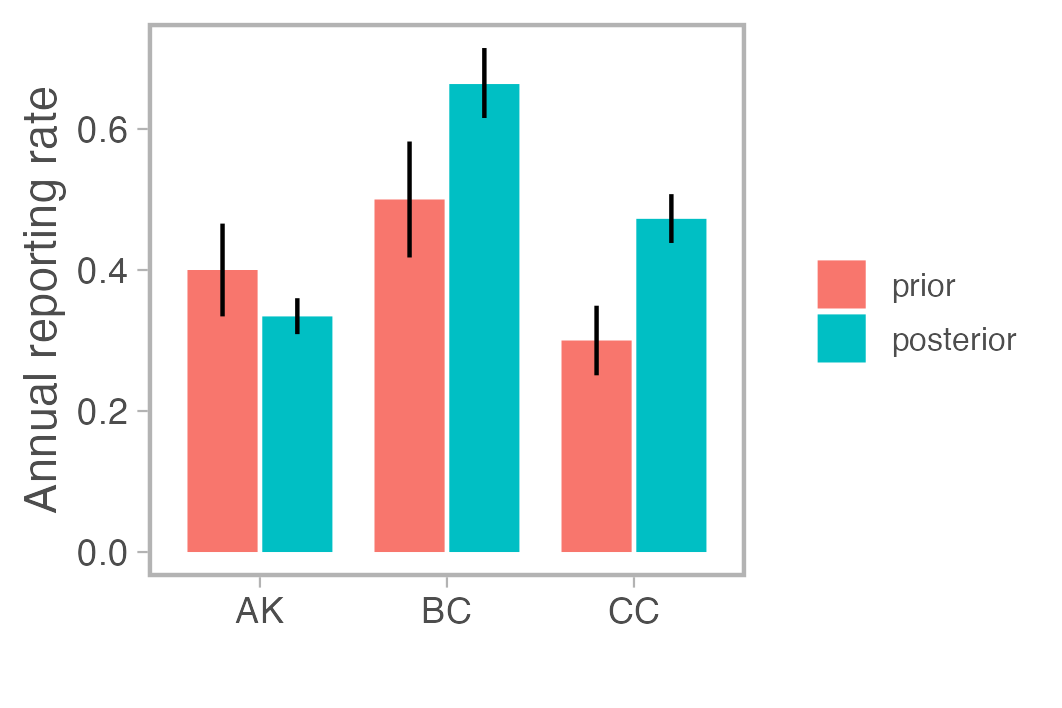
\includegraphics[width = 0.7\textwidth]{bar-regions-3-reporting-priors-posteriors}
    \caption{TBD}
    \label{fig:bar-regions-3-reporting-priors-posteriors}
\end{figure}

\begin{figure}[htb]
    \centering
    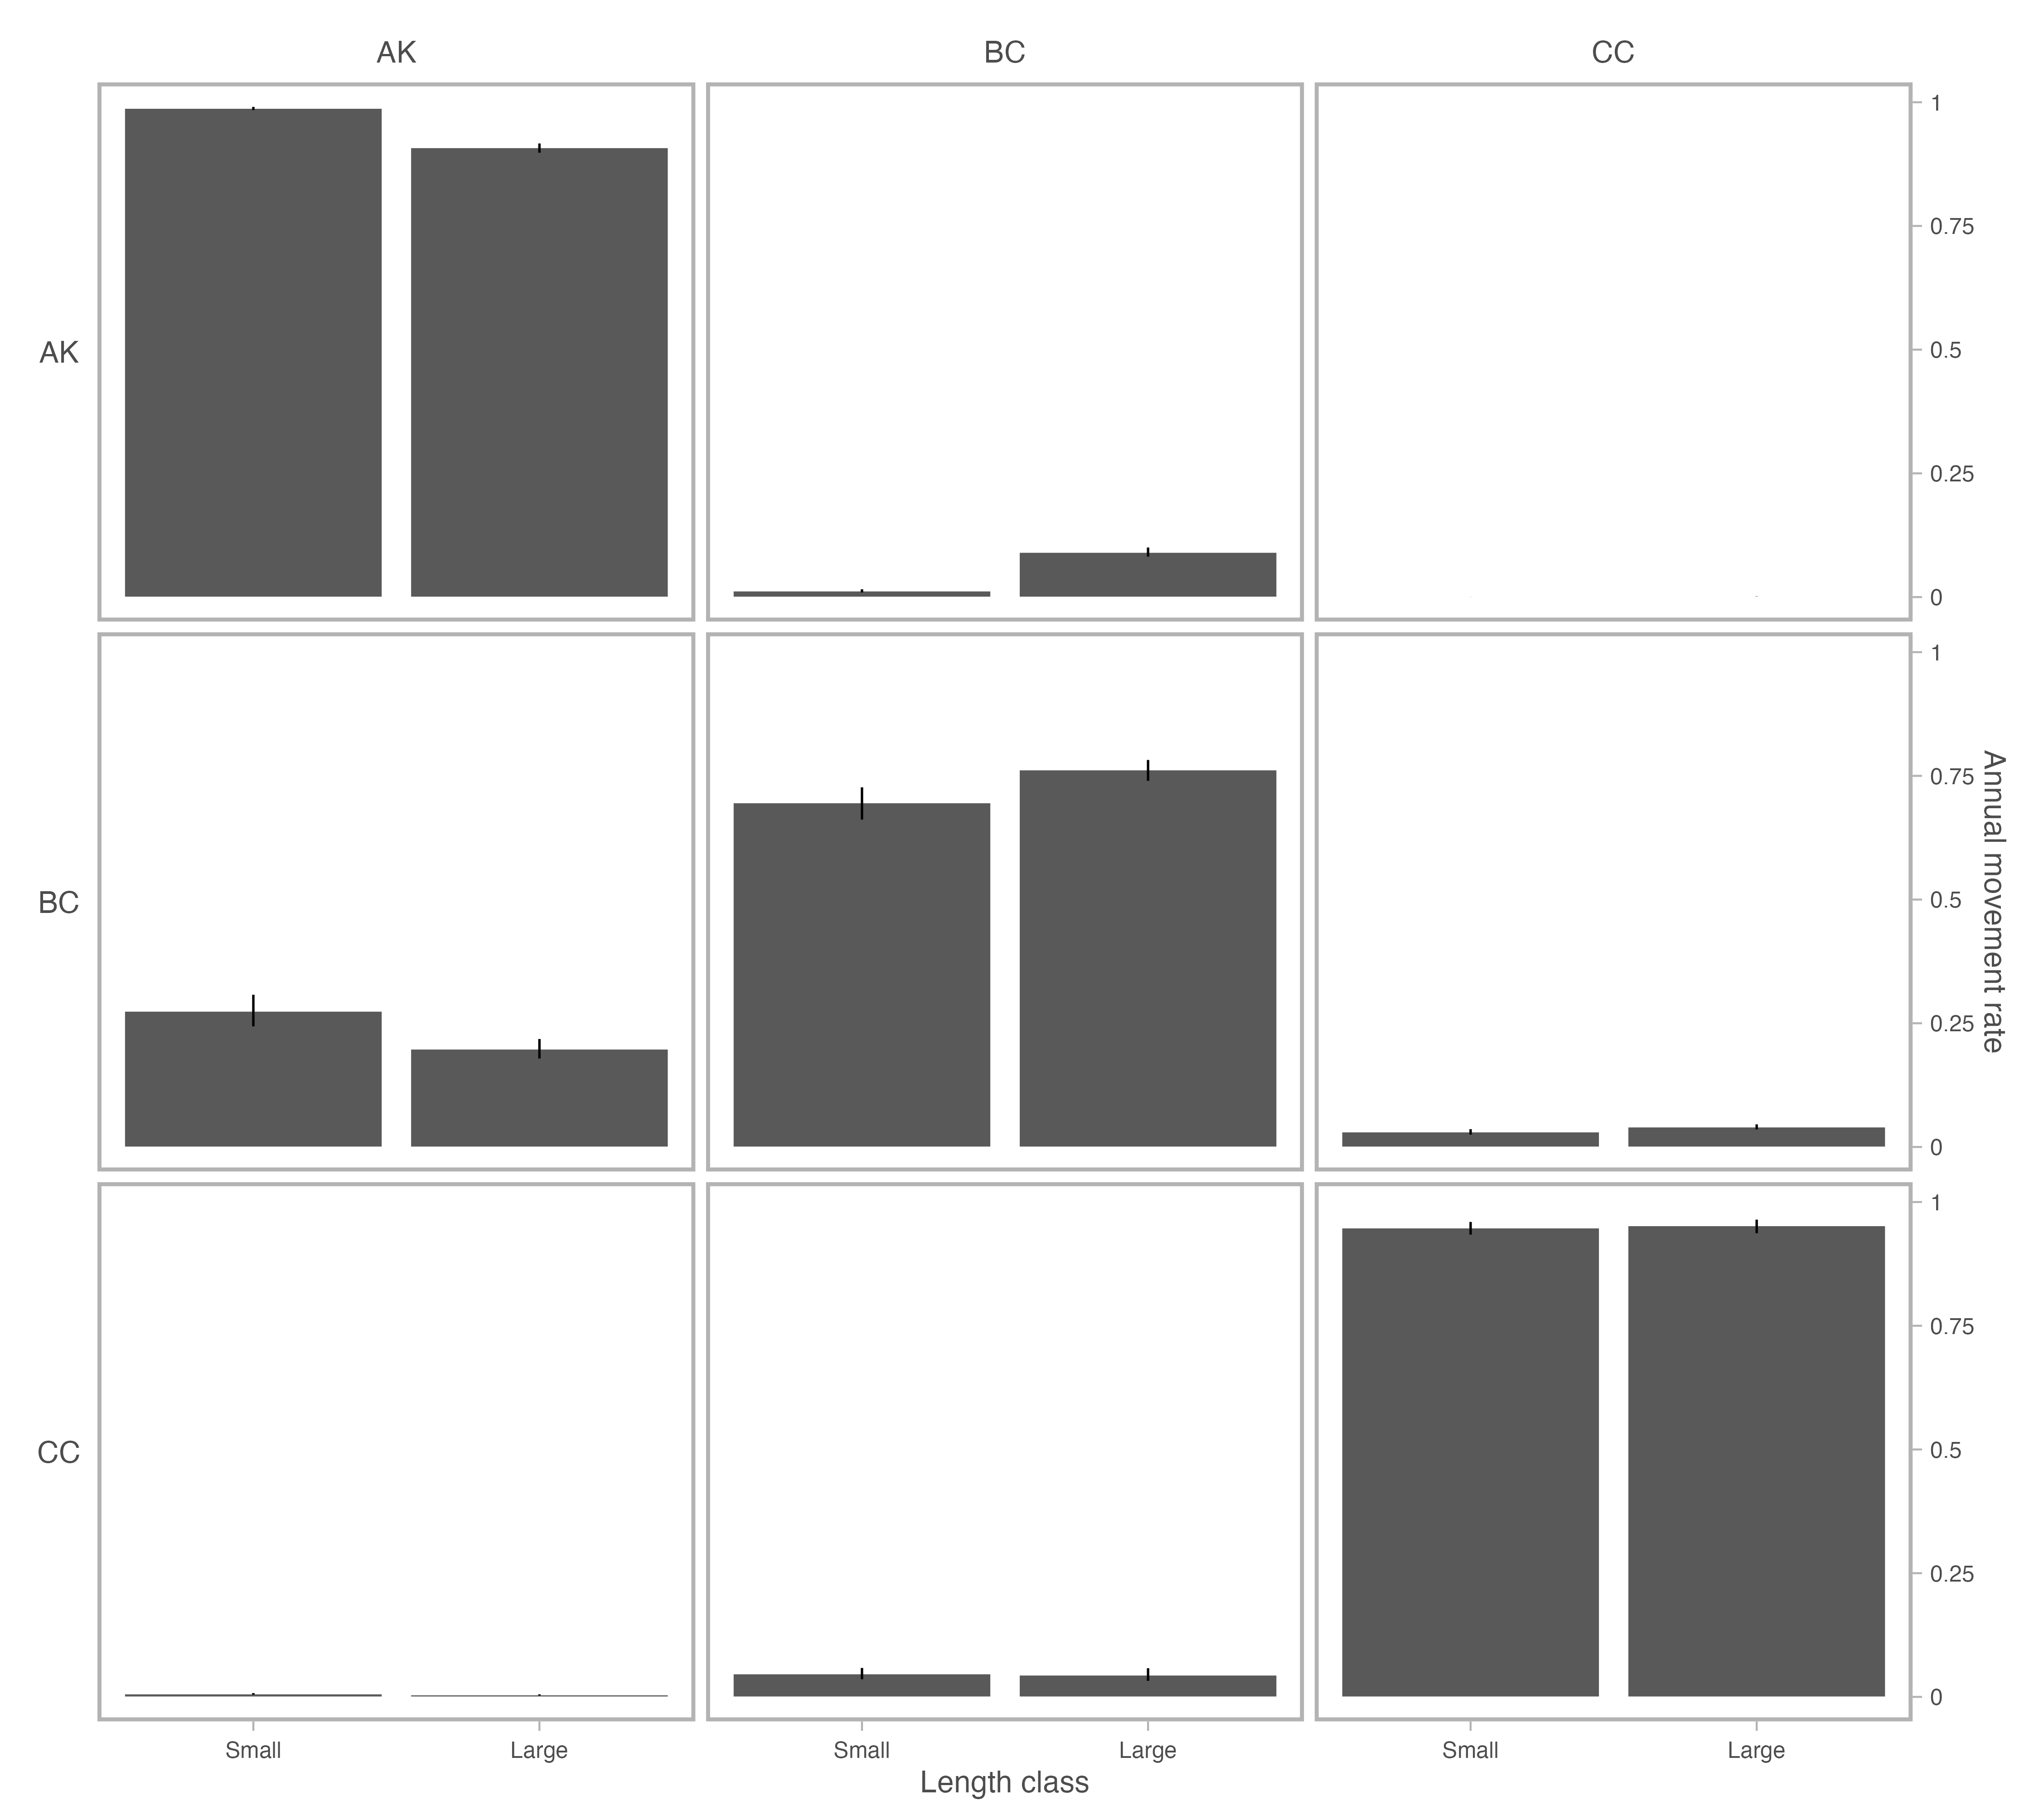
\includegraphics[width = 0.7\textwidth]{bar-regions-3-size}
    \caption{TBD}
    \label{fig:bar-regions-3-size}
\end{figure}

\begin{figure}[htb]
    \centering
    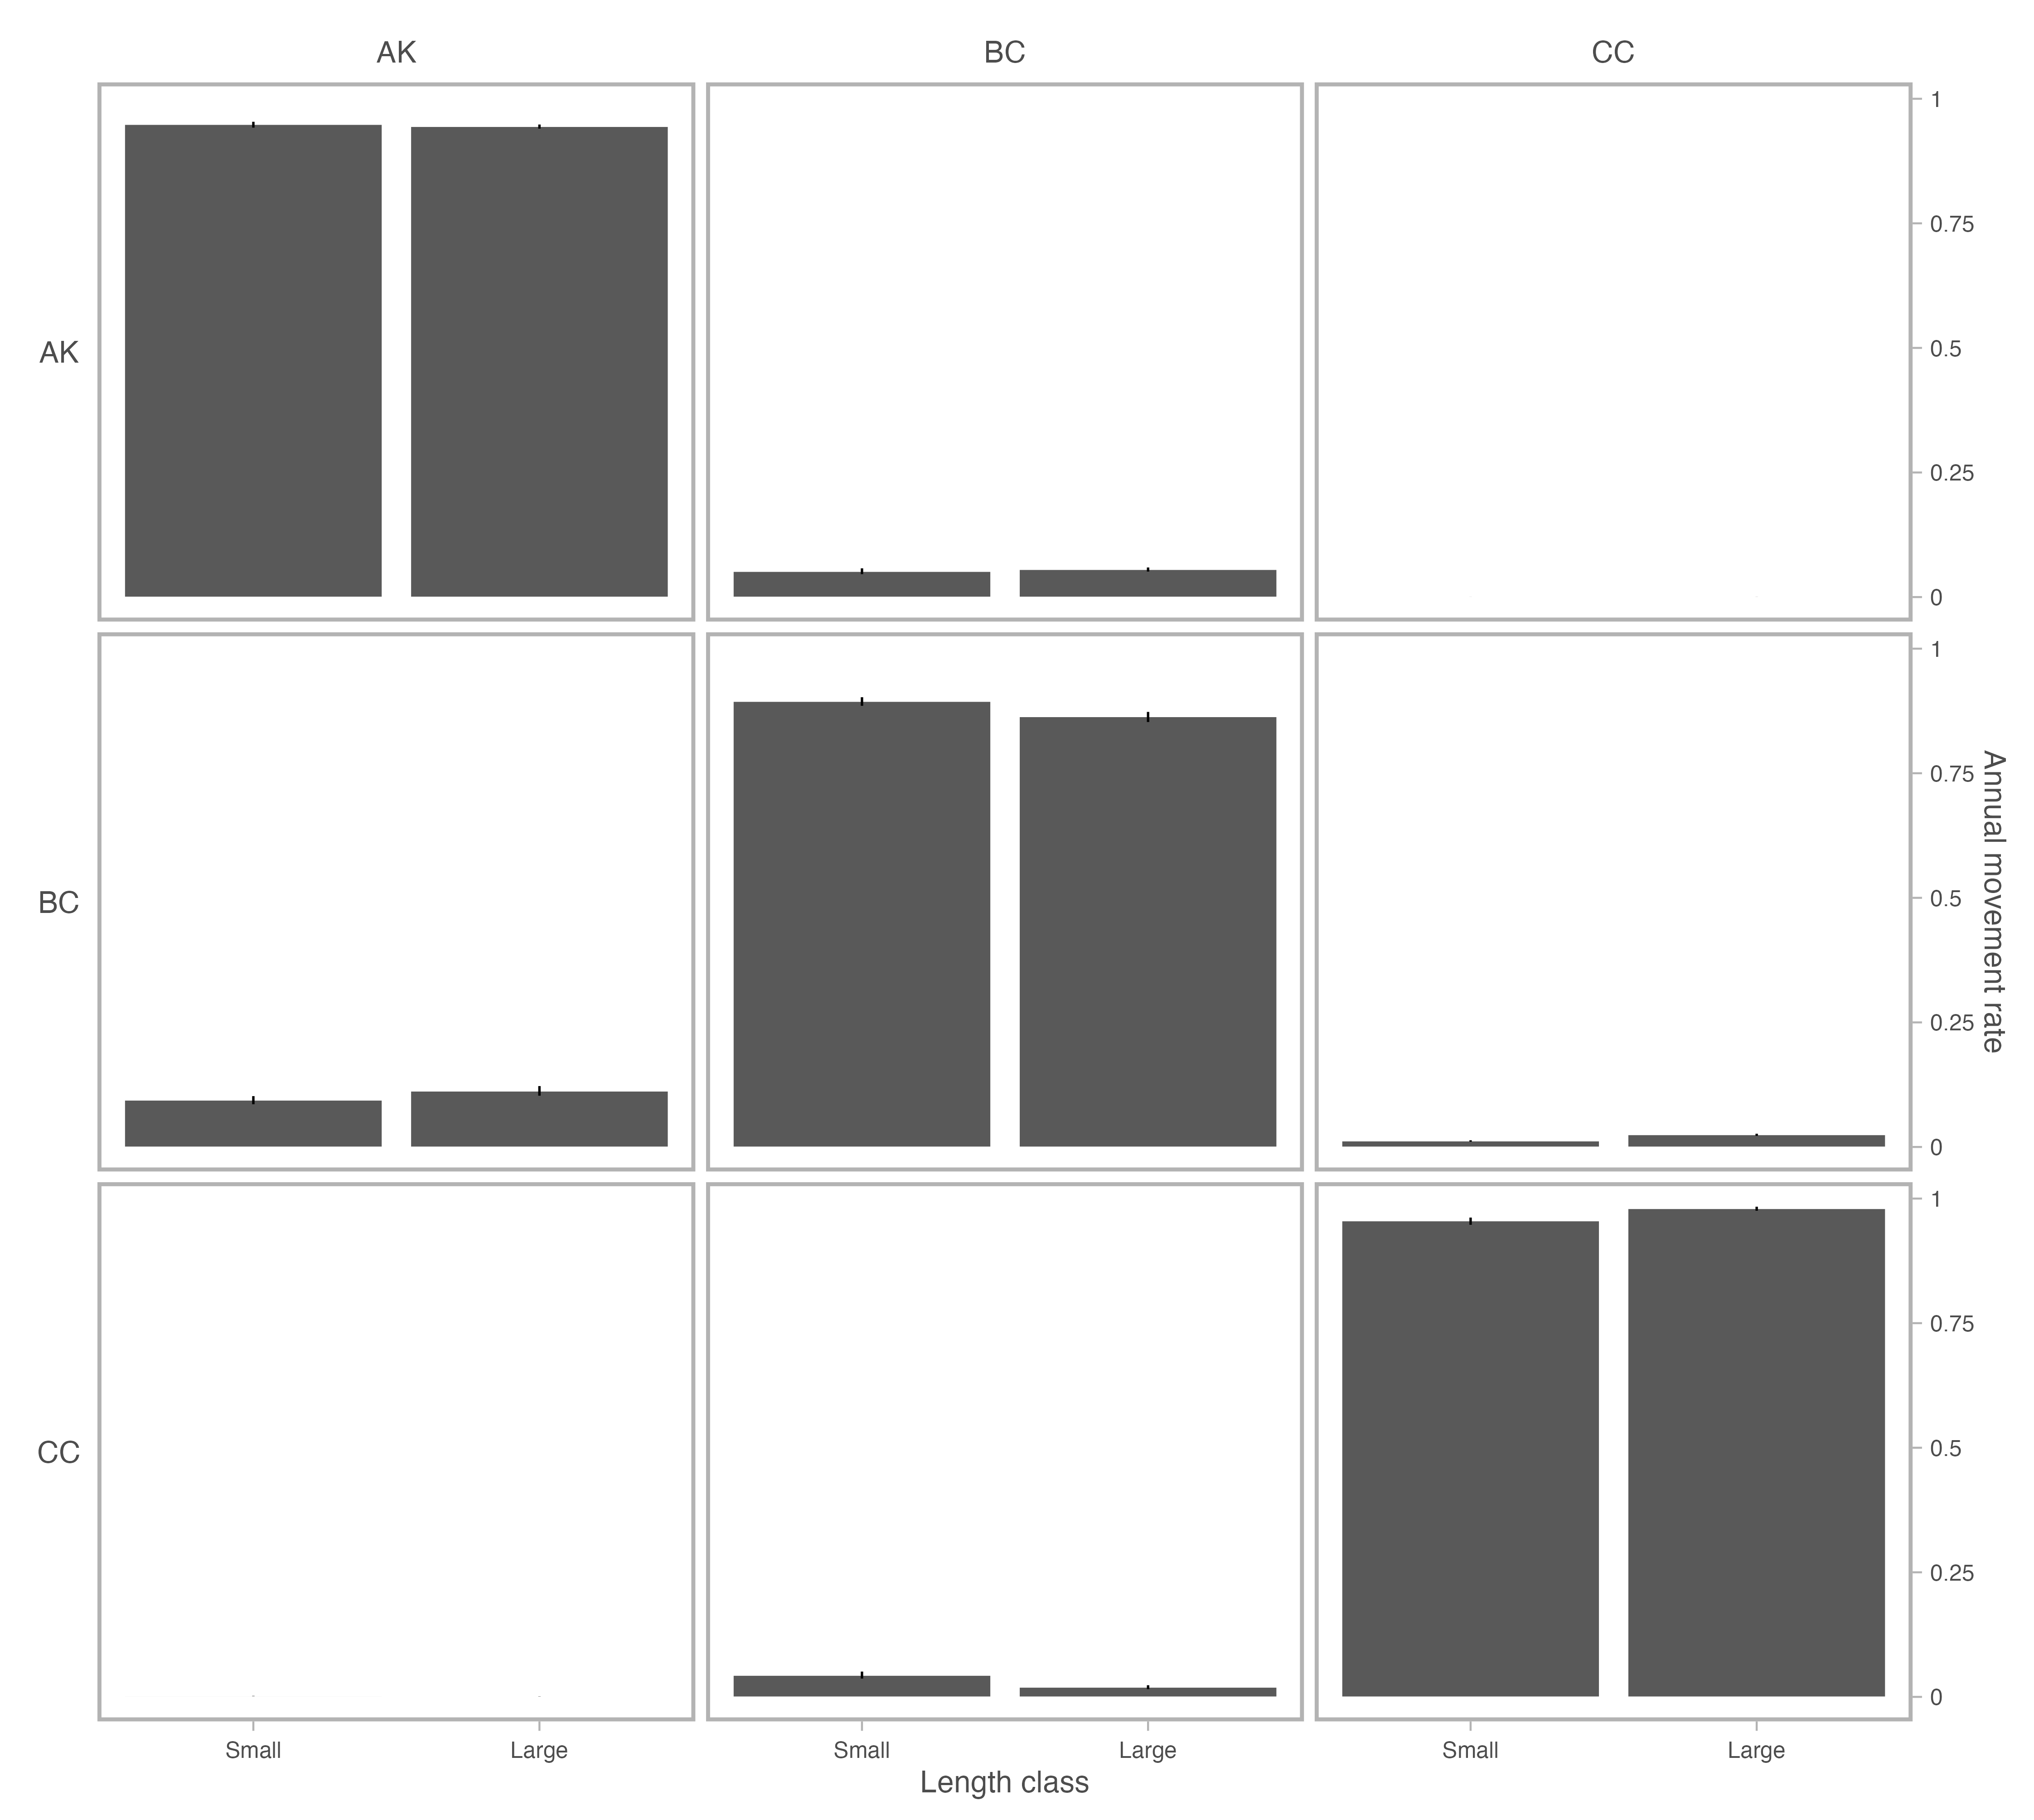
\includegraphics[width = 0.7\textwidth]{bar-regions-3-size-no-duration-constraint}
    \caption{TBD}
    \label{fig:bar-regions-3-size-no-duration-constraint}
\end{figure}

\begin{figure}[htb]
    \centering
    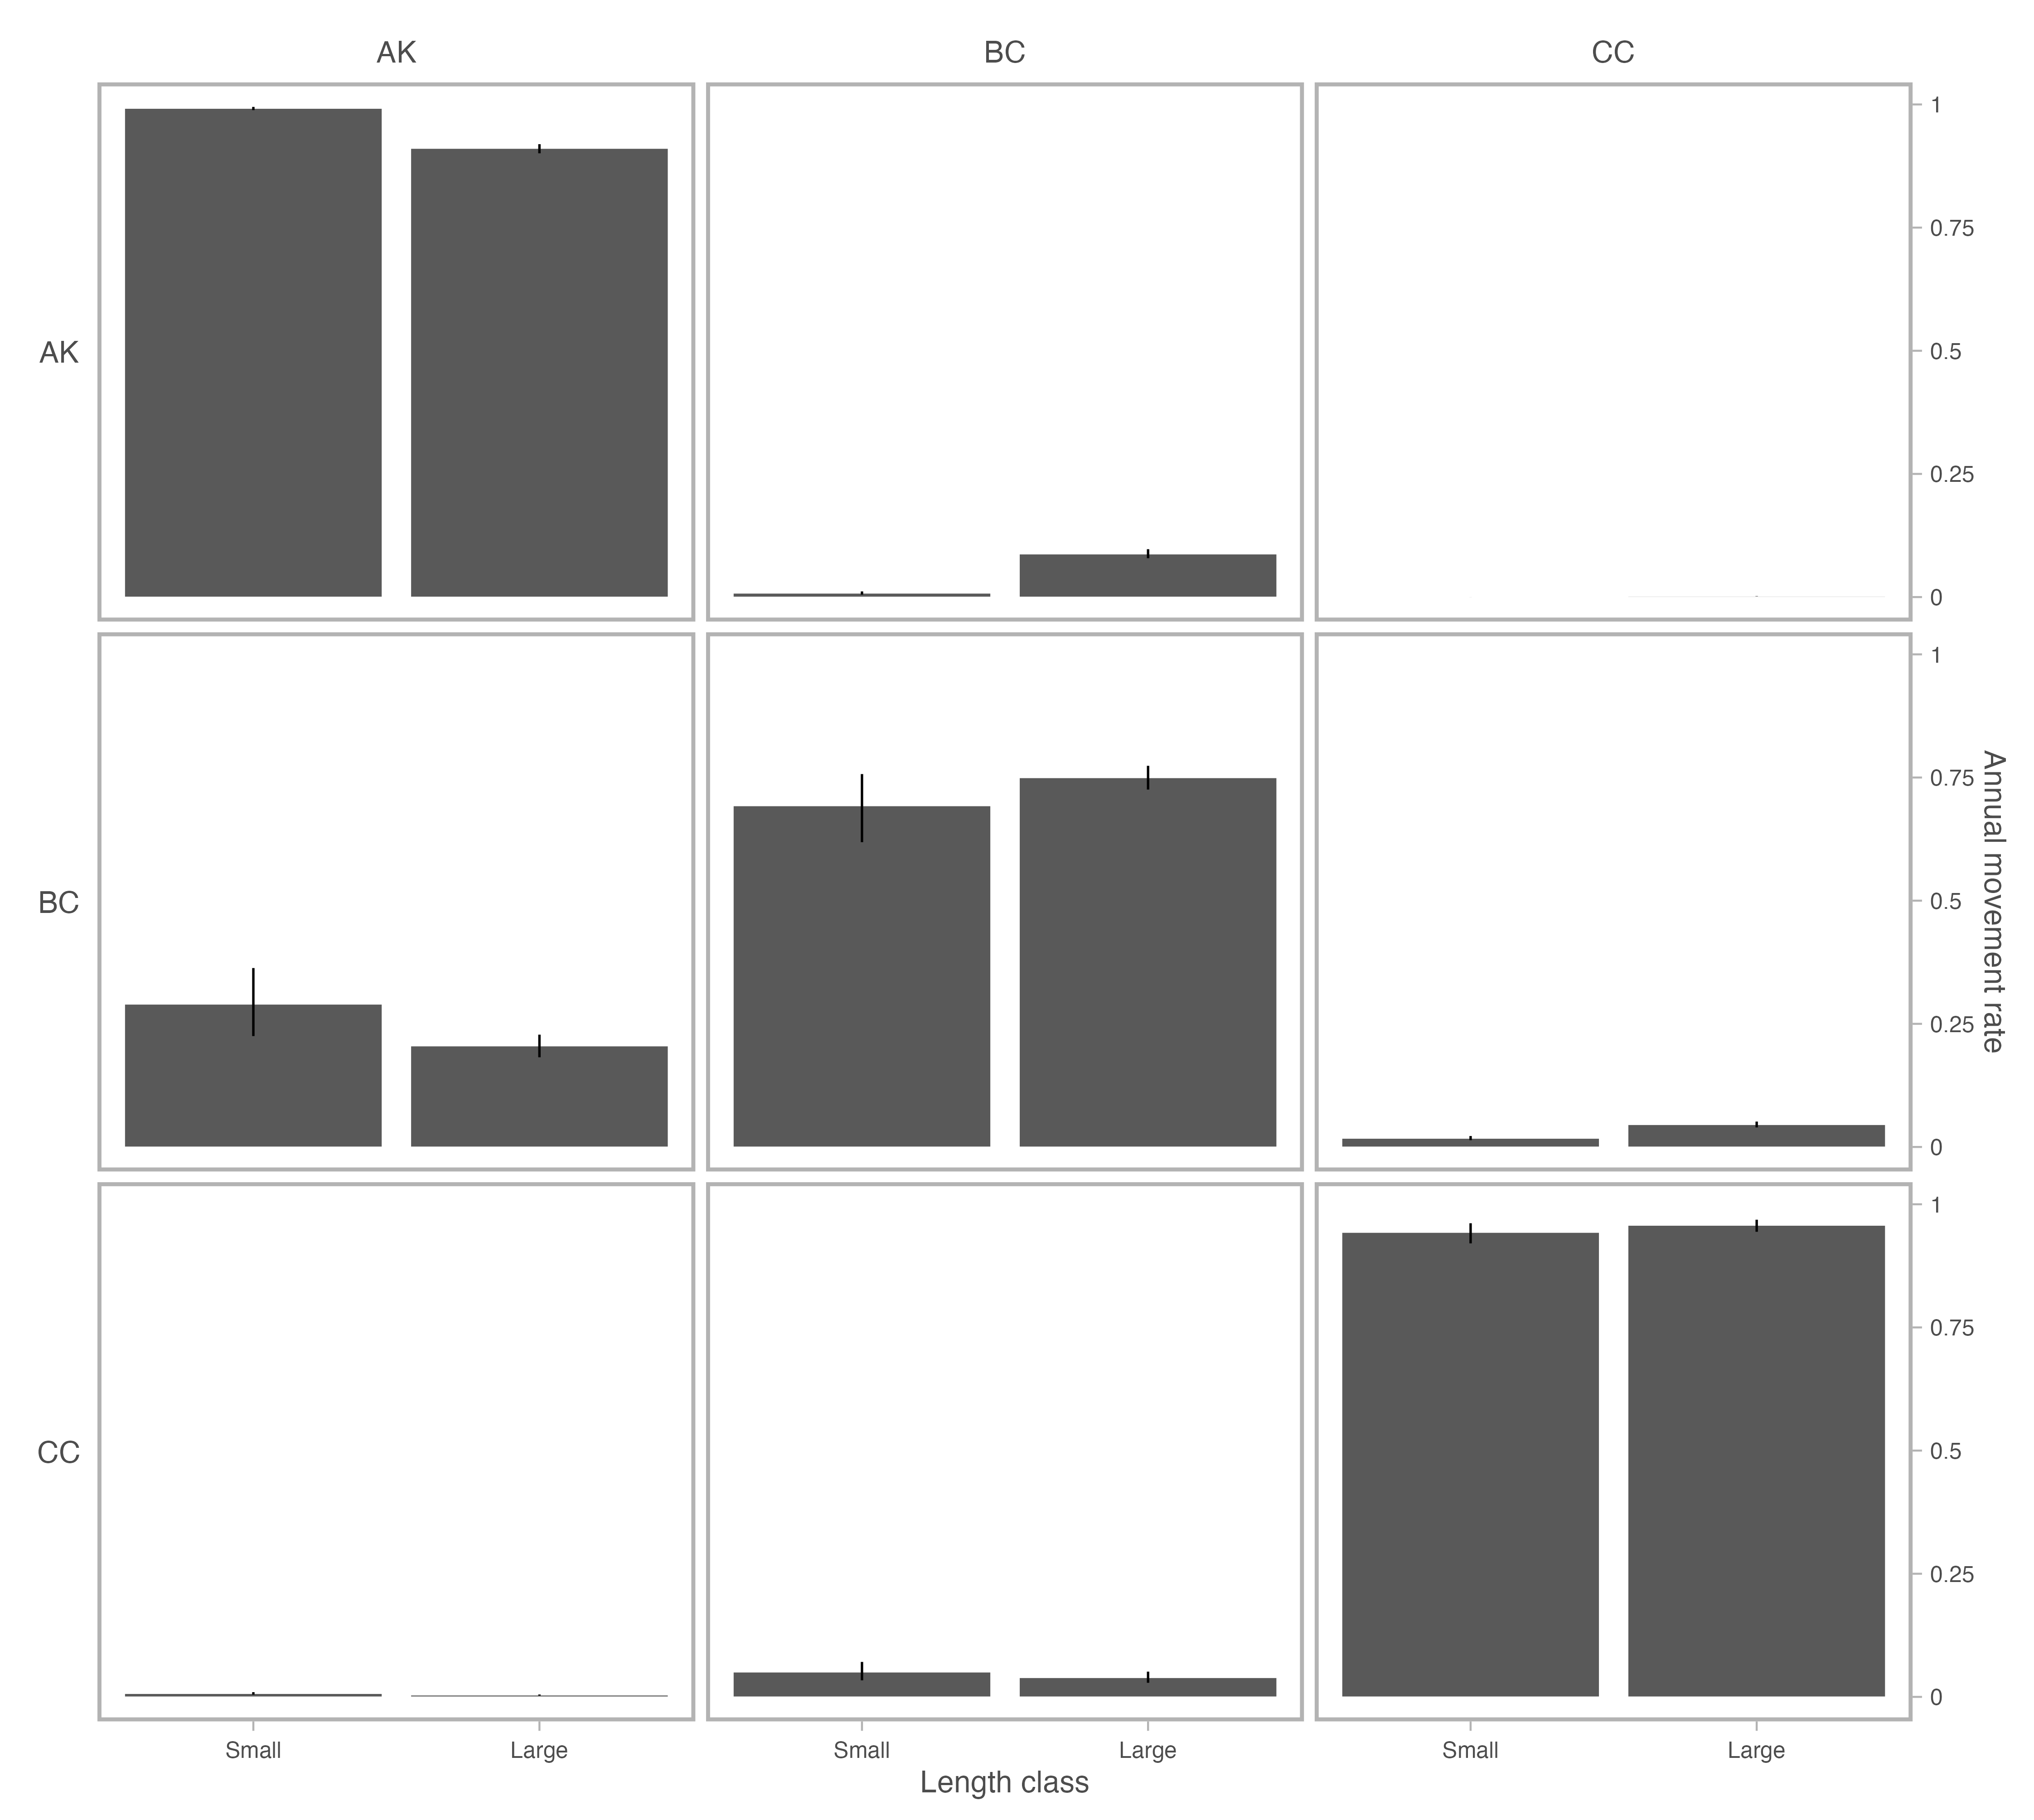
\includegraphics[width = 0.7\textwidth]{bar-regions-3-size-no-recovery-transition}
    \caption{TBD}
    \label{fig:bar-regions-3-size-no-recovery-transition}
\end{figure}




\newpage
\bibliography{refs}

% End
\end{document}







